\appendix
\chapter{Evidencias de la aplicación en el emulador}
Las figuras de este apéndice son las capturas originales del directorio de evidencias. Se conservaron sus nombres para que coincidan con \texttt{resultados.json}. El archivo 03 tiene el mismo hash que el 02 en el registro existente.

\begin{figure}[!htbp]\centering
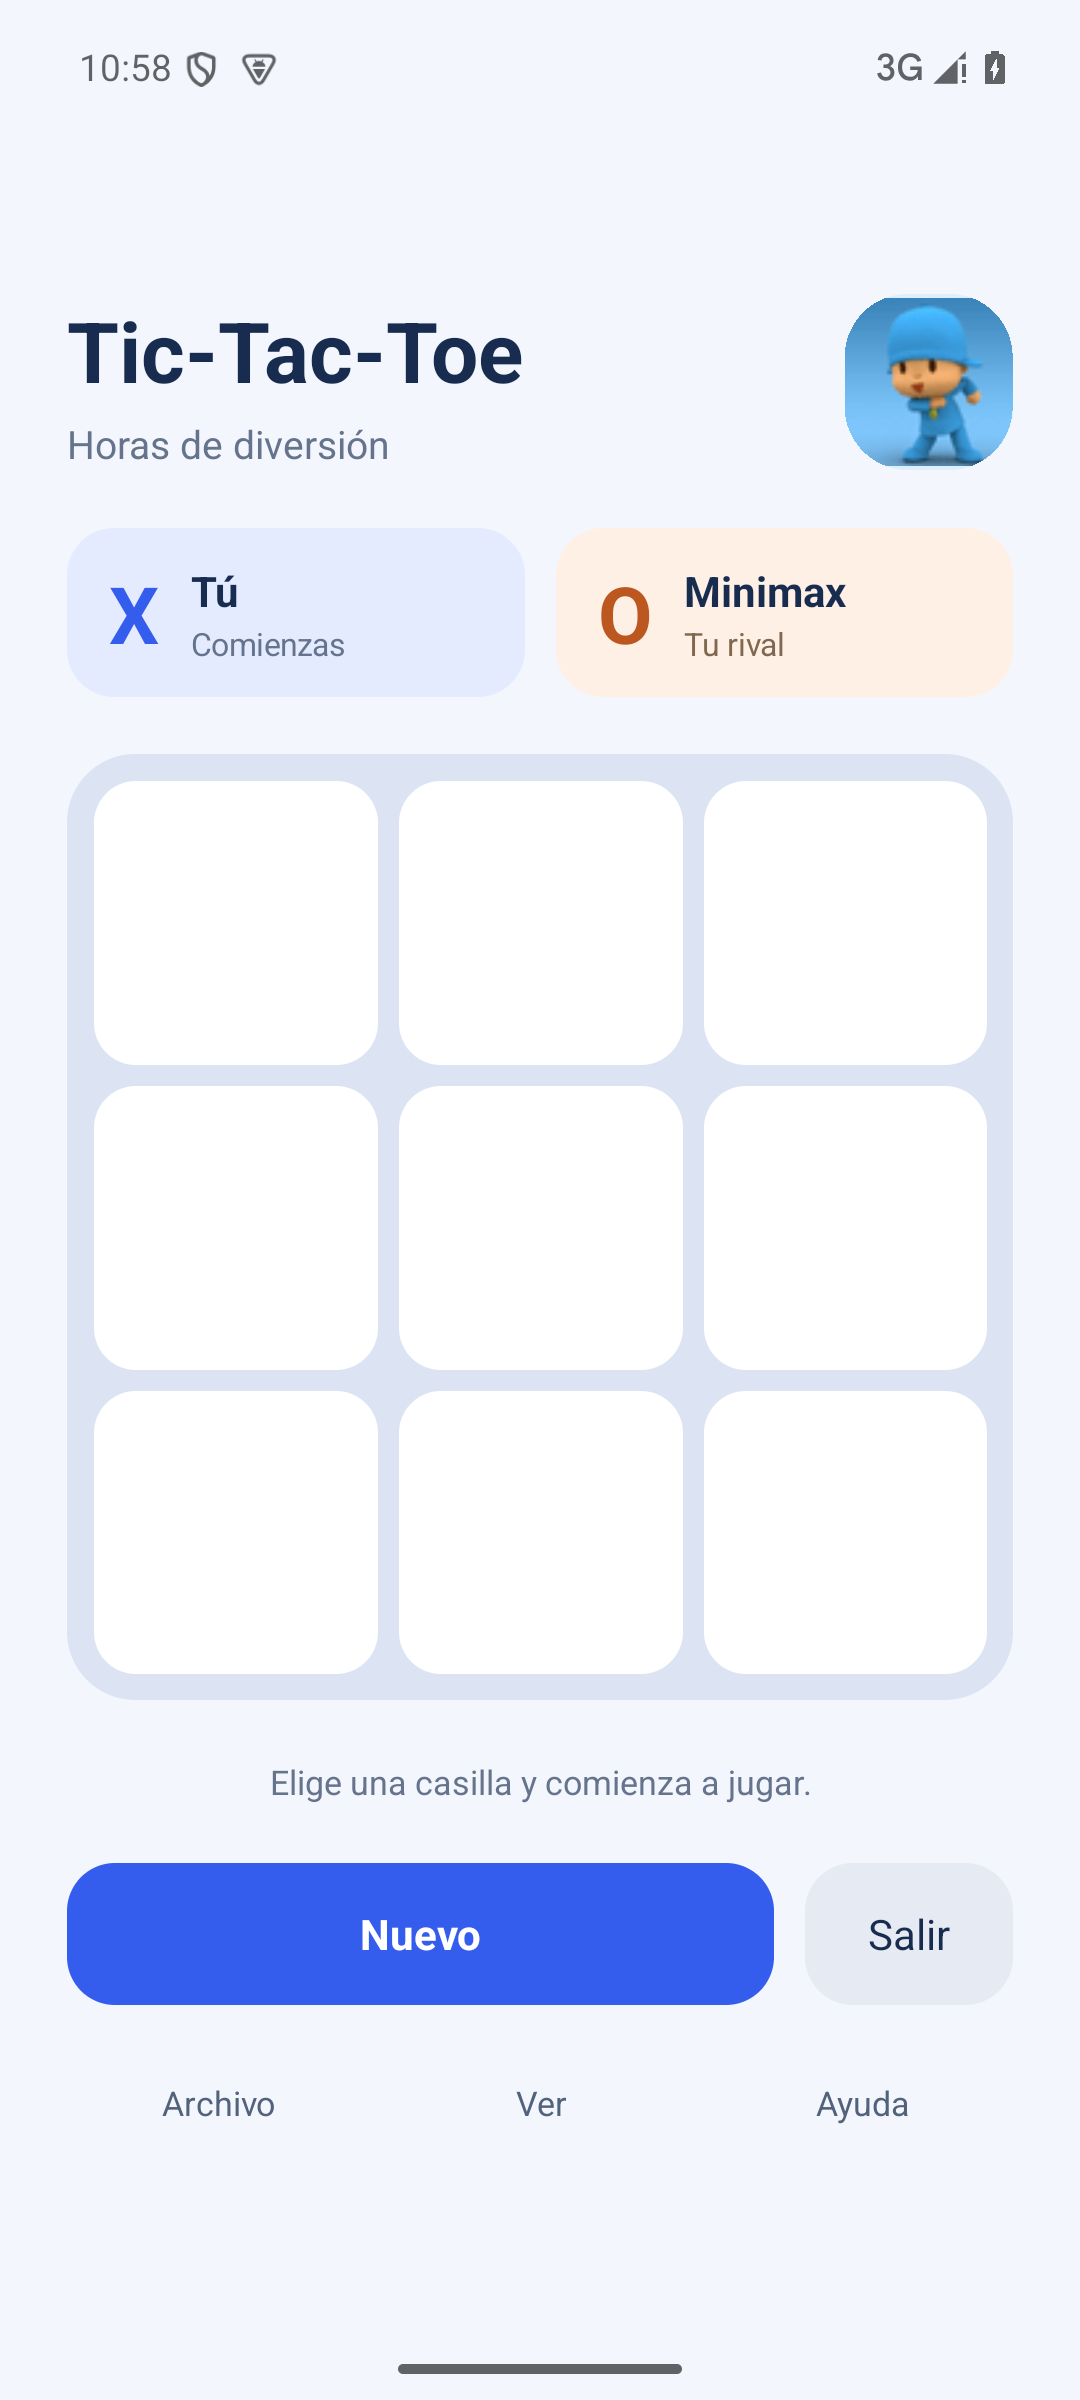
\includegraphics[height=0.78\textheight,keepaspectratio]{figuras/emulador/01_inicio.png}
\caption{Pantalla inicial con el tablero vacío, los símbolos de cada participante y los controles visibles.}\label{fig:emu01}
\end{figure}
\clearpage
\begin{figure}[!htbp]\centering
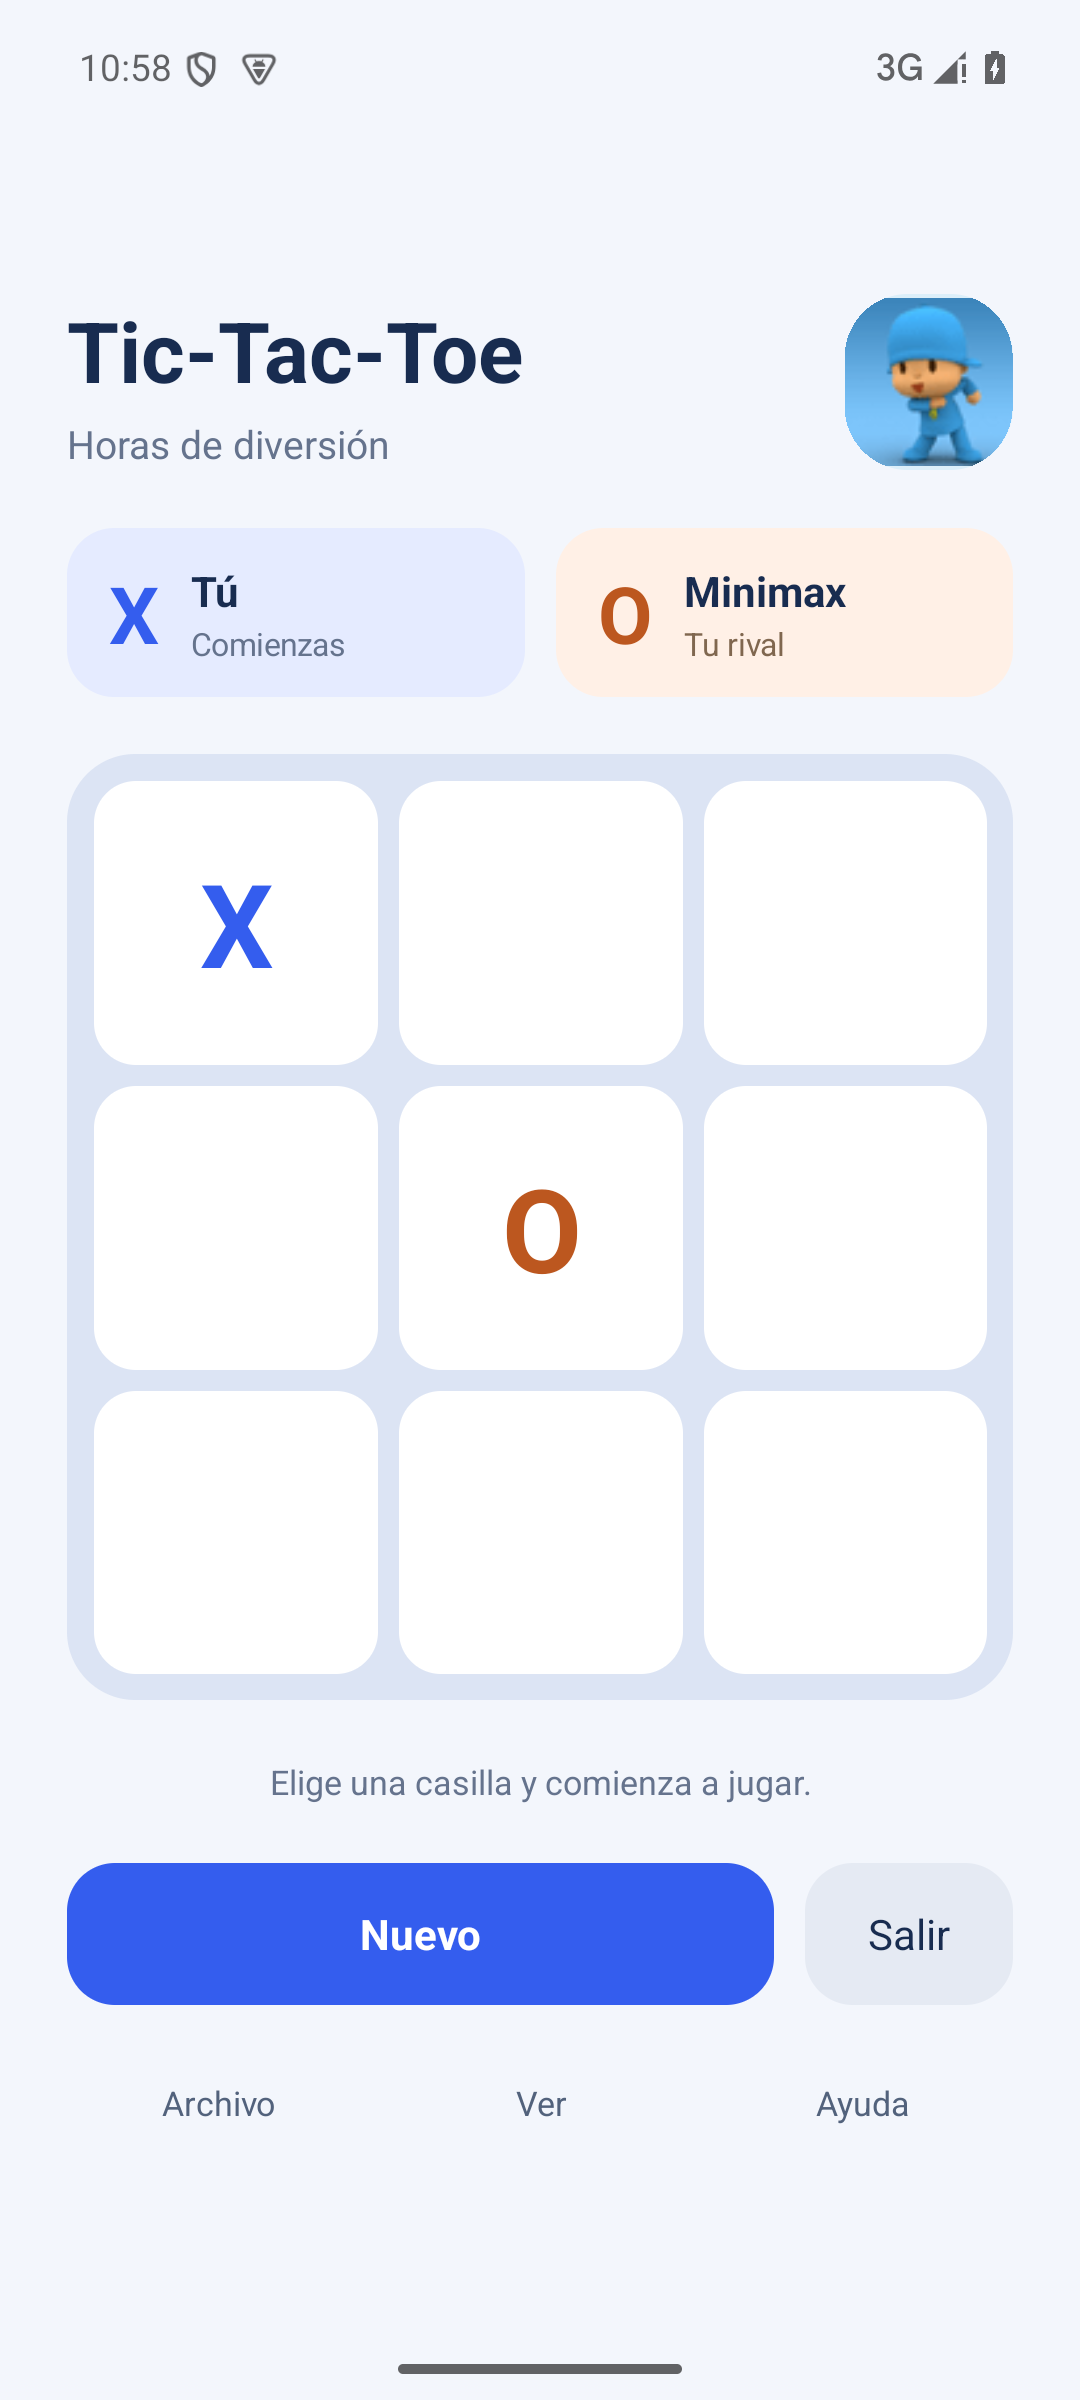
\includegraphics[height=0.78\textheight,keepaspectratio]{figuras/emulador/02_turno_humano_ia.png}
\caption{La persona coloca \texttt{X} y Minimax responde con \texttt{O}.}\label{fig:emu02}
\end{figure}
\clearpage
\begin{figure}[!htbp]\centering
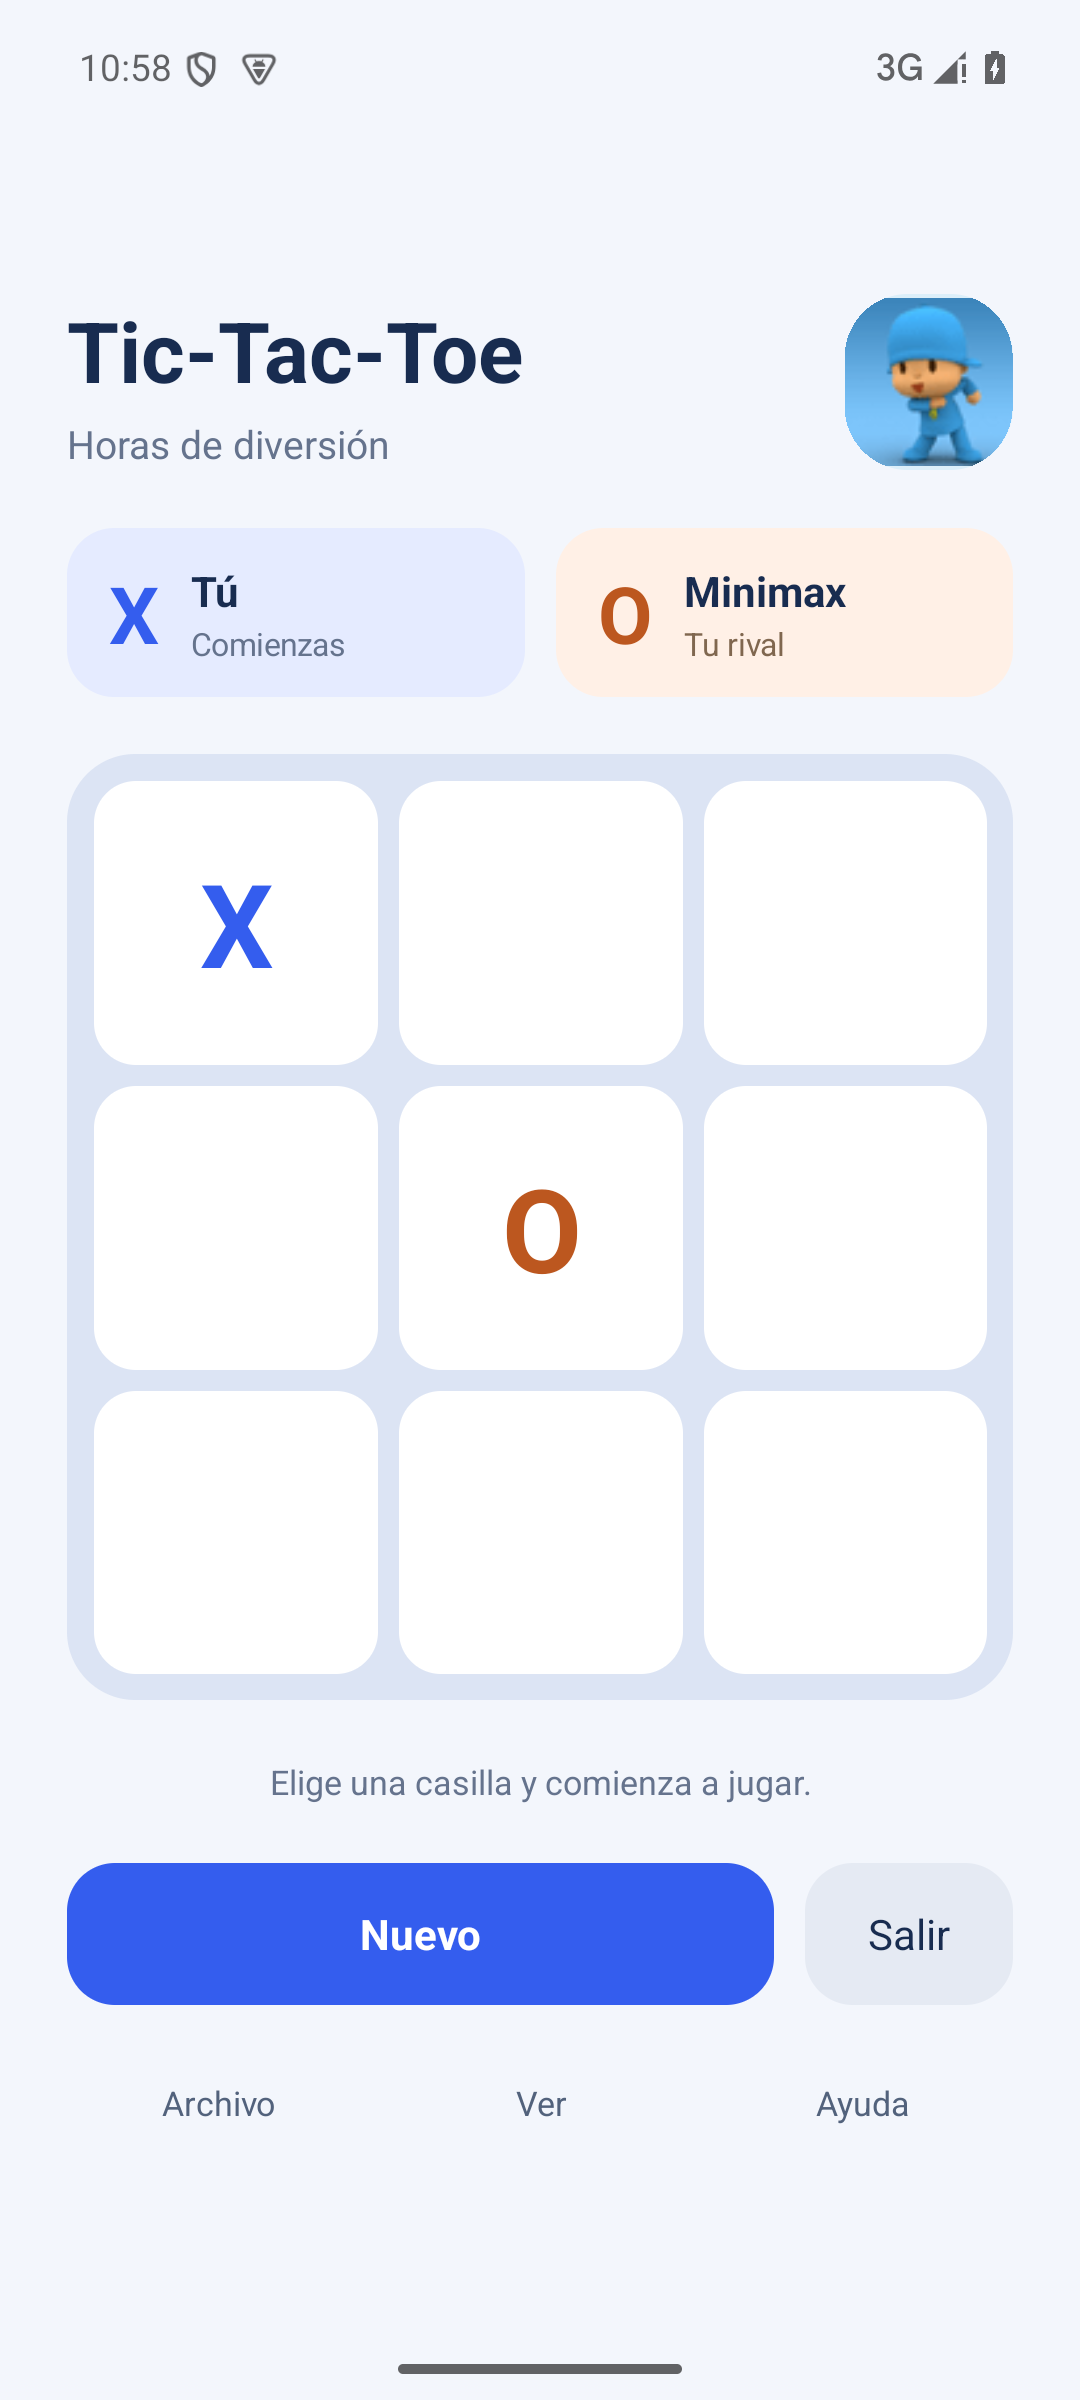
\includegraphics[height=0.78\textheight,keepaspectratio]{figuras/emulador/03_casilla_ocupada.png}
\caption{Verificación registrada para la casilla ocupada; la imagen conserva el mismo hash que la captura 02.}\label{fig:emu03}
\end{figure}
\clearpage
\begin{figure}[!htbp]\centering
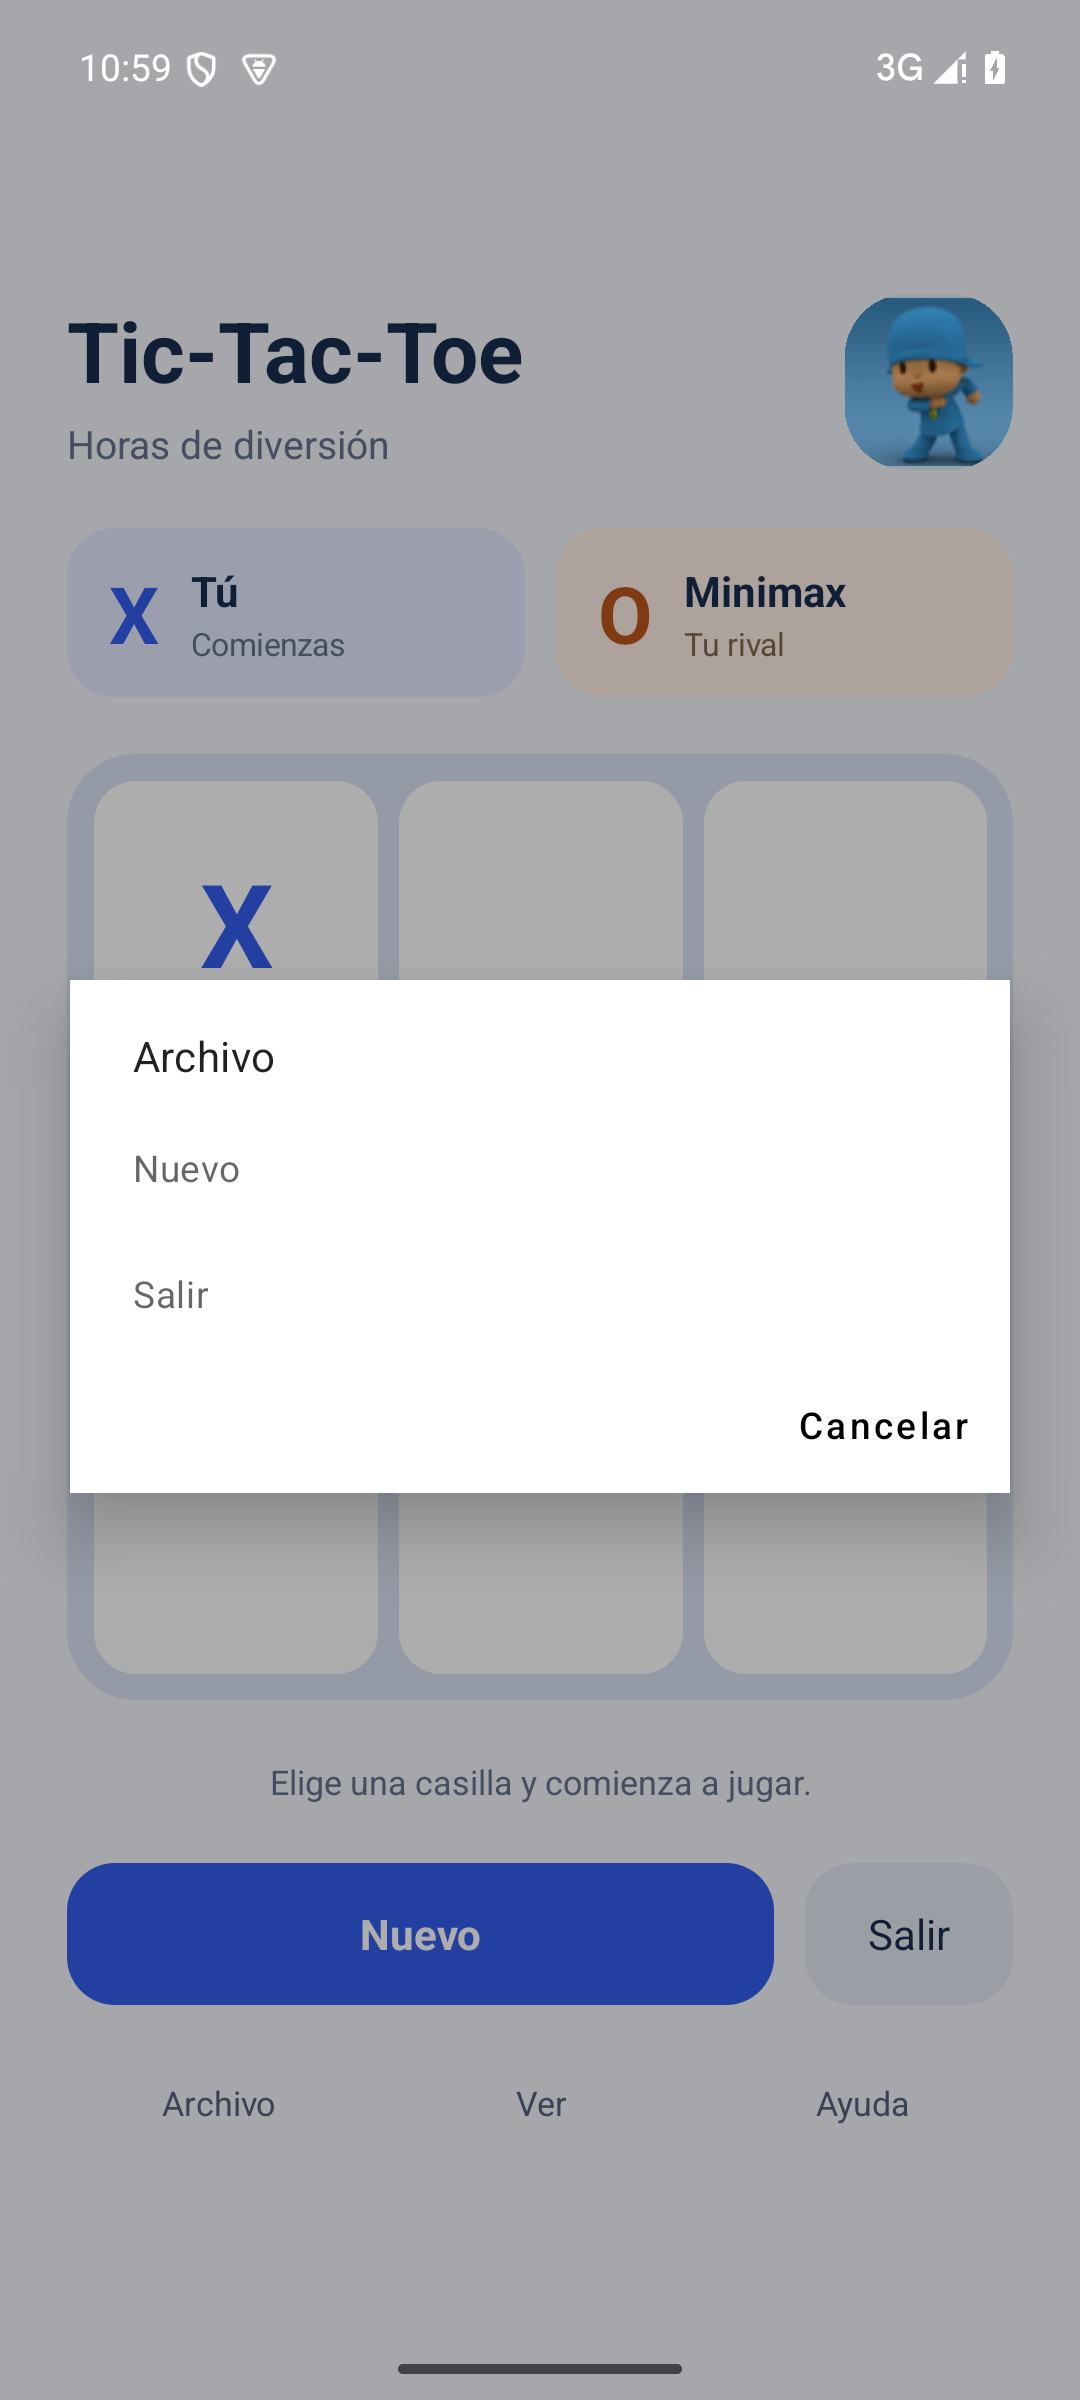
\includegraphics[height=0.78\textheight,keepaspectratio]{figuras/emulador/04_menu_archivo.png}
\caption{Hoja de acciones del menú Archivo. Las opciones no están conectadas a manejadores de acción.}\label{fig:emu04}
\end{figure}
\clearpage
\begin{figure}[!htbp]\centering
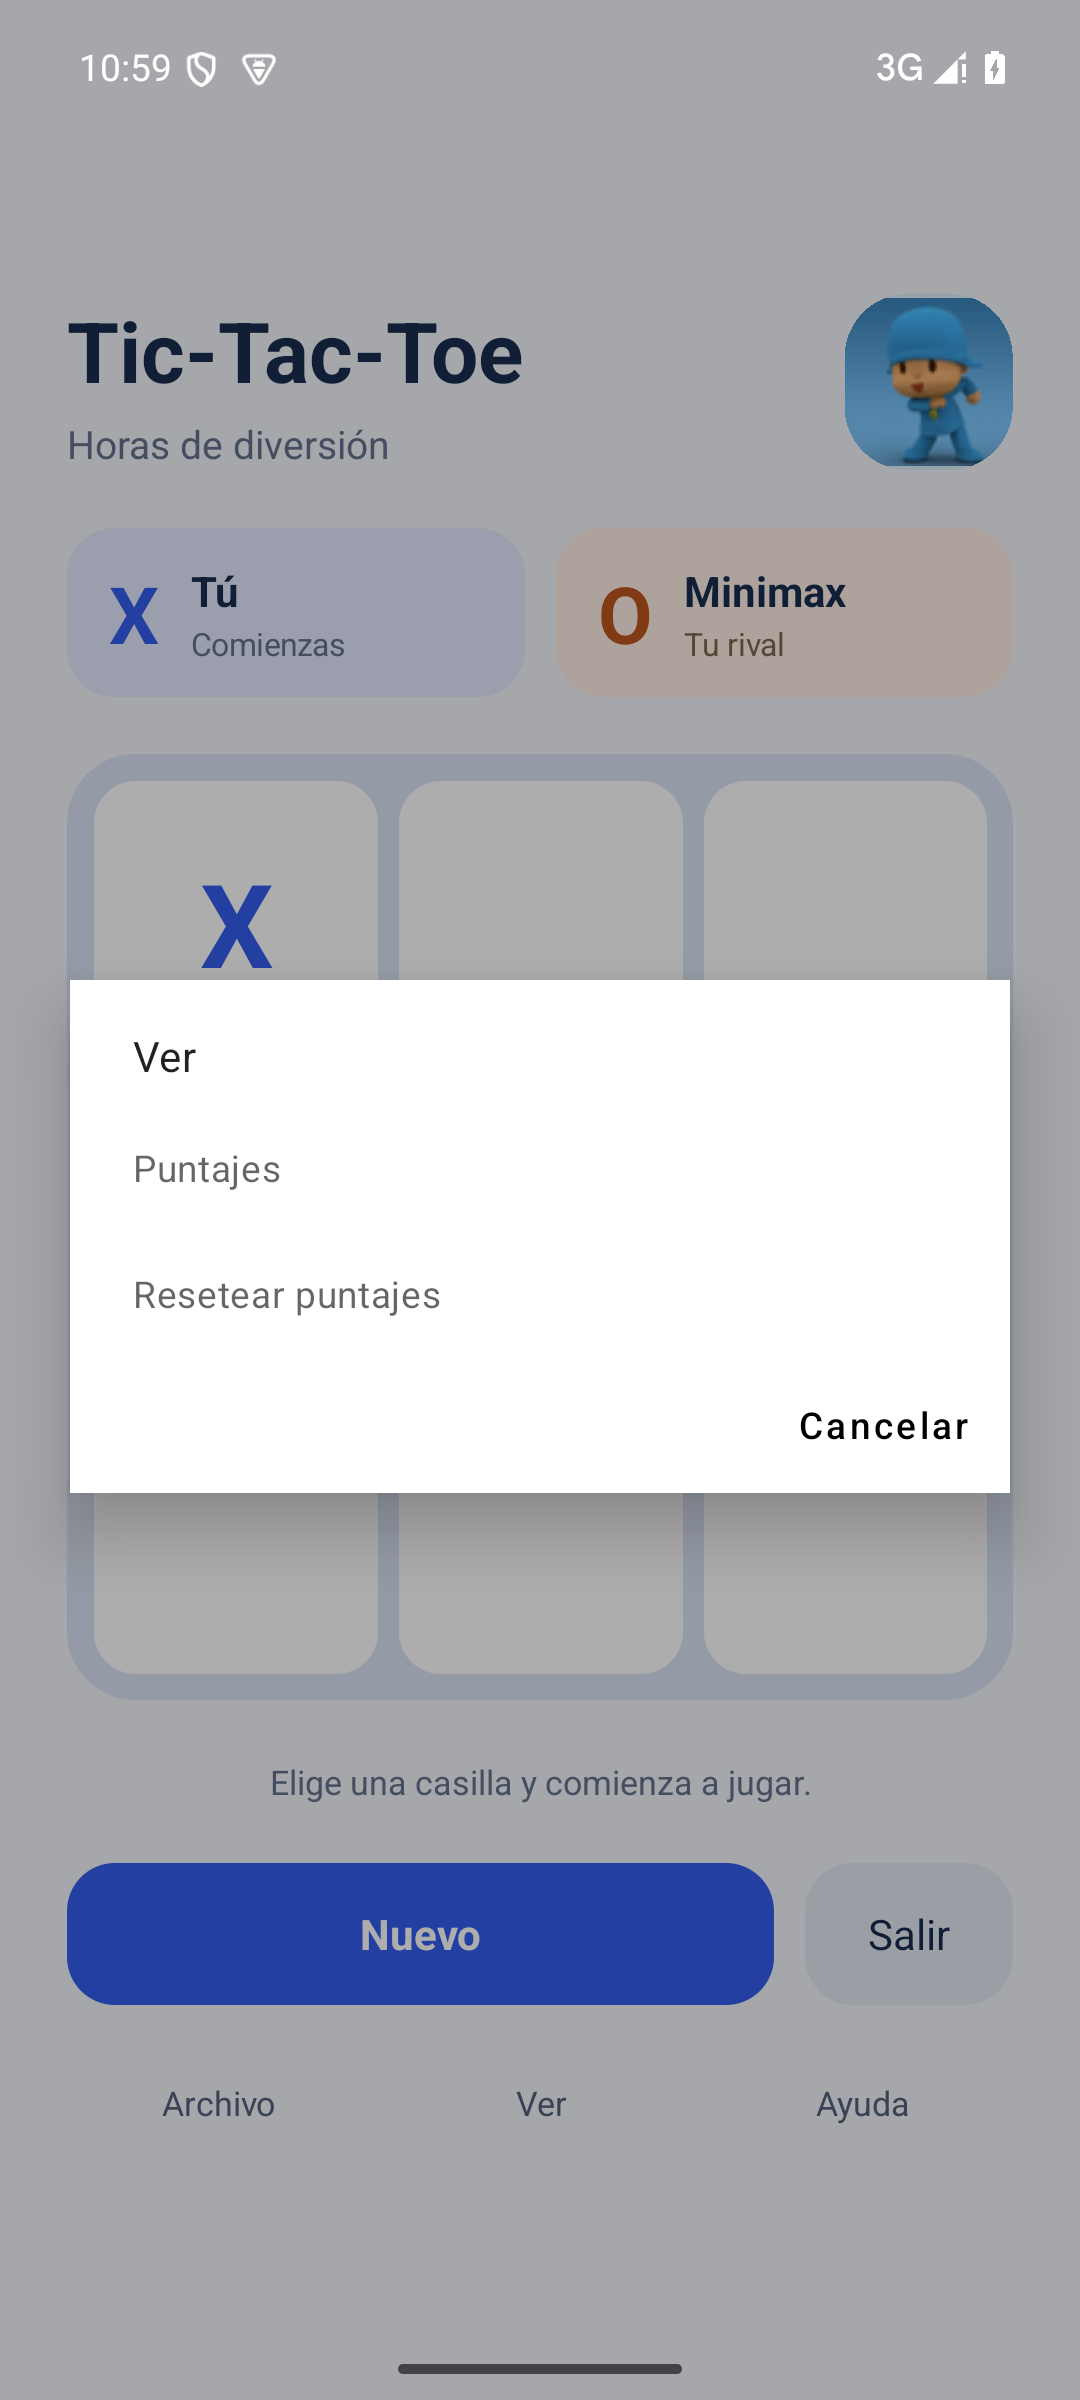
\includegraphics[height=0.78\textheight,keepaspectratio]{figuras/emulador/05_menu_ver.png}
\caption{Hoja de acciones del menú Ver. Puntajes y Resetear puntajes son etiquetas visibles, sin función implementada.}\label{fig:emu05}
\end{figure}
\clearpage
\begin{figure}[!htbp]\centering
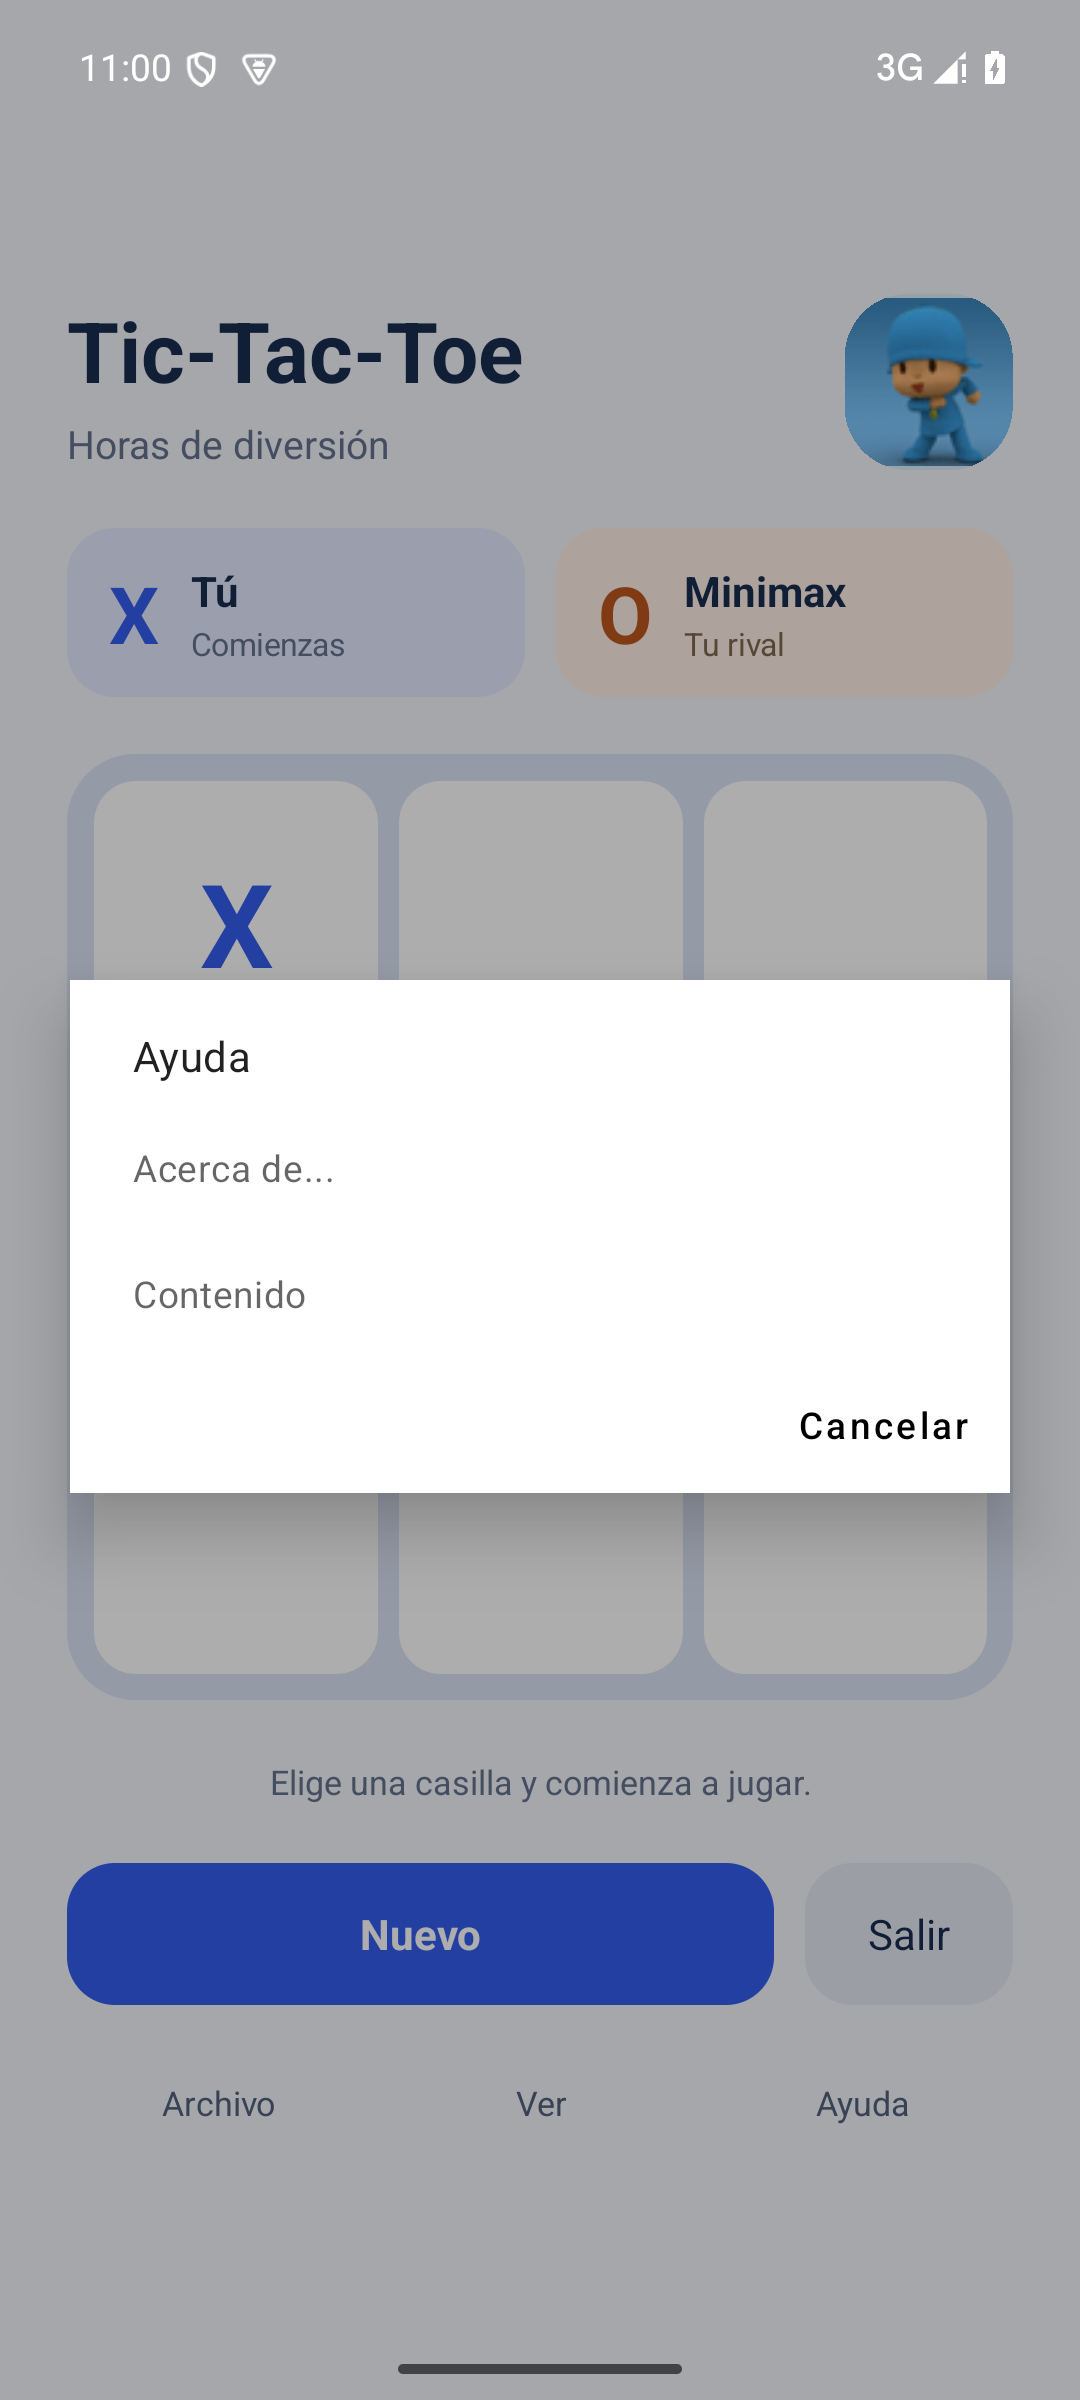
\includegraphics[height=0.78\textheight,keepaspectratio]{figuras/emulador/06_menu_ayuda.png}
\caption{Hoja de acciones del menú Ayuda; las selecciones no abren contenido.}\label{fig:emu06}
\end{figure}
\clearpage
\begin{figure}[!htbp]\centering
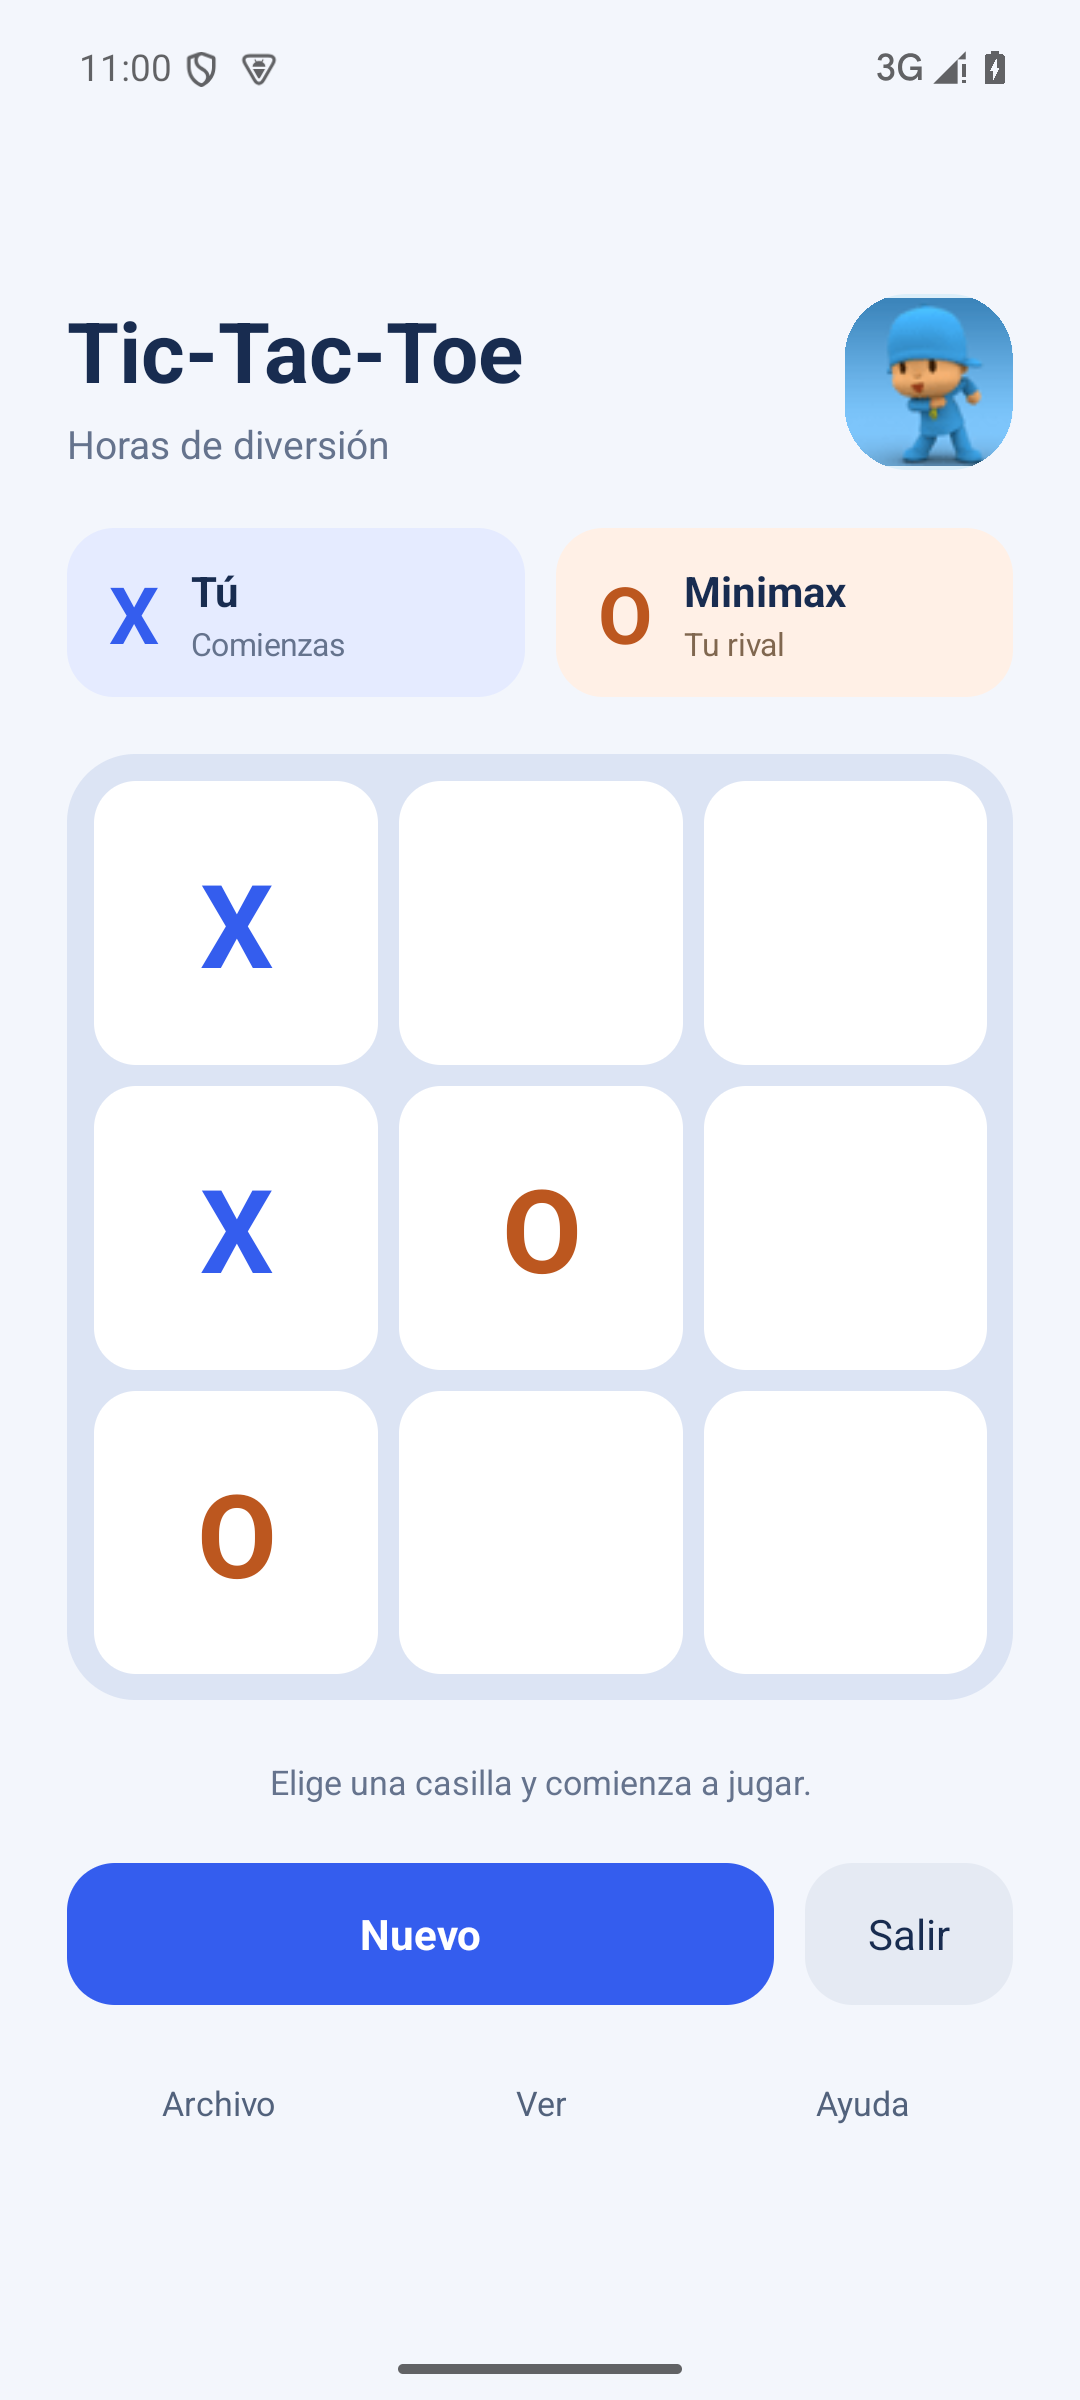
\includegraphics[height=0.78\textheight,keepaspectratio]{figuras/emulador/07_ia_bloquea.png}
\caption{Minimax bloquea la amenaza de victoria de \texttt{X} en la primera columna.}\label{fig:emu07}
\end{figure}
\clearpage
\begin{figure}[!htbp]\centering
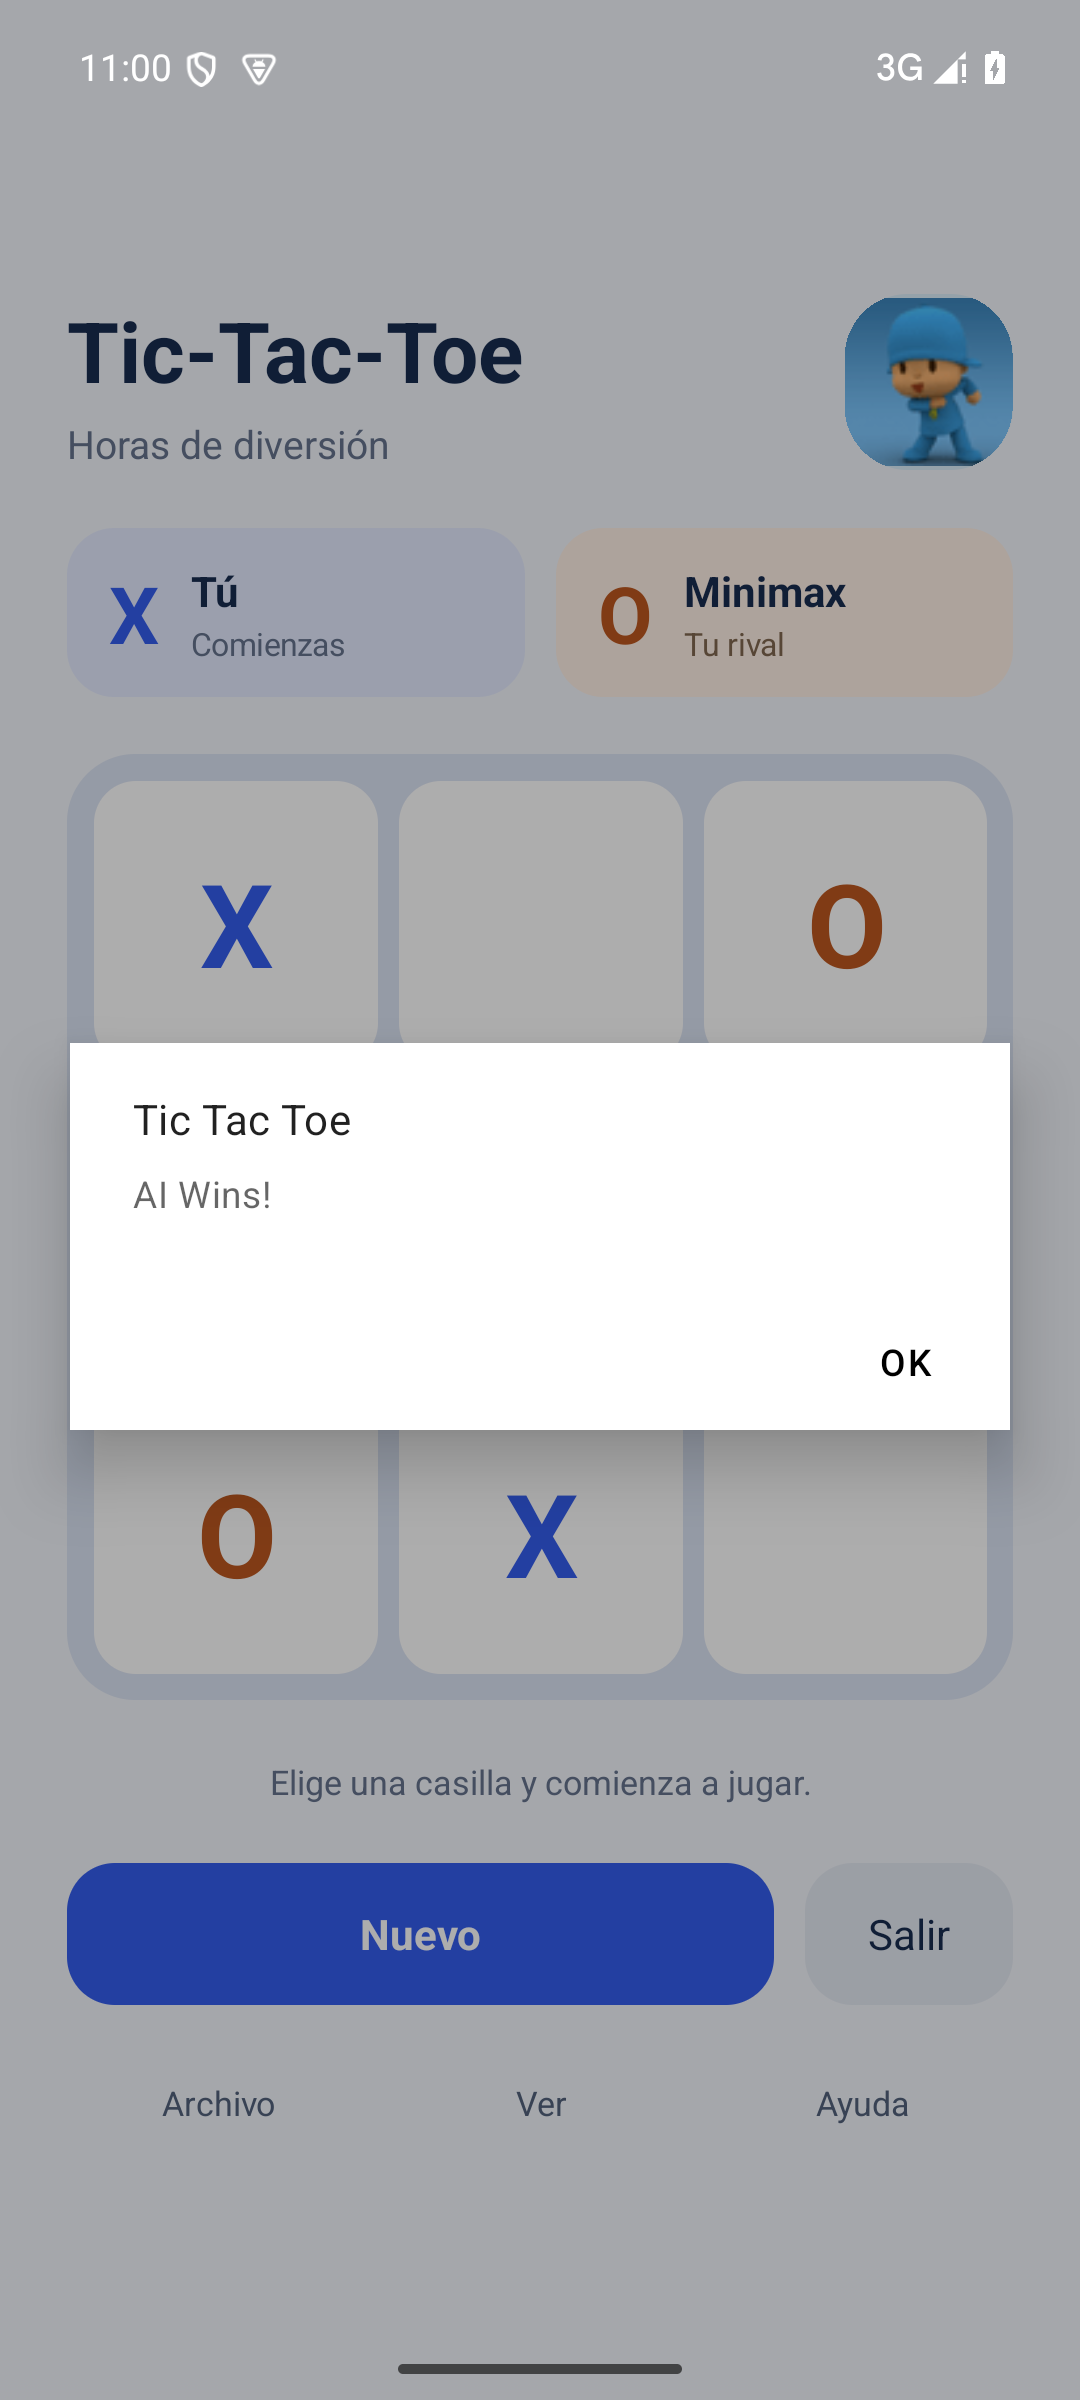
\includegraphics[height=0.78\textheight,keepaspectratio]{figuras/emulador/08_victoria_ia.png}
\caption{Aviso de victoria de la IA registrado en el escenario de prueba.}\label{fig:emu08}
\end{figure}
\clearpage
\begin{figure}[!htbp]\centering
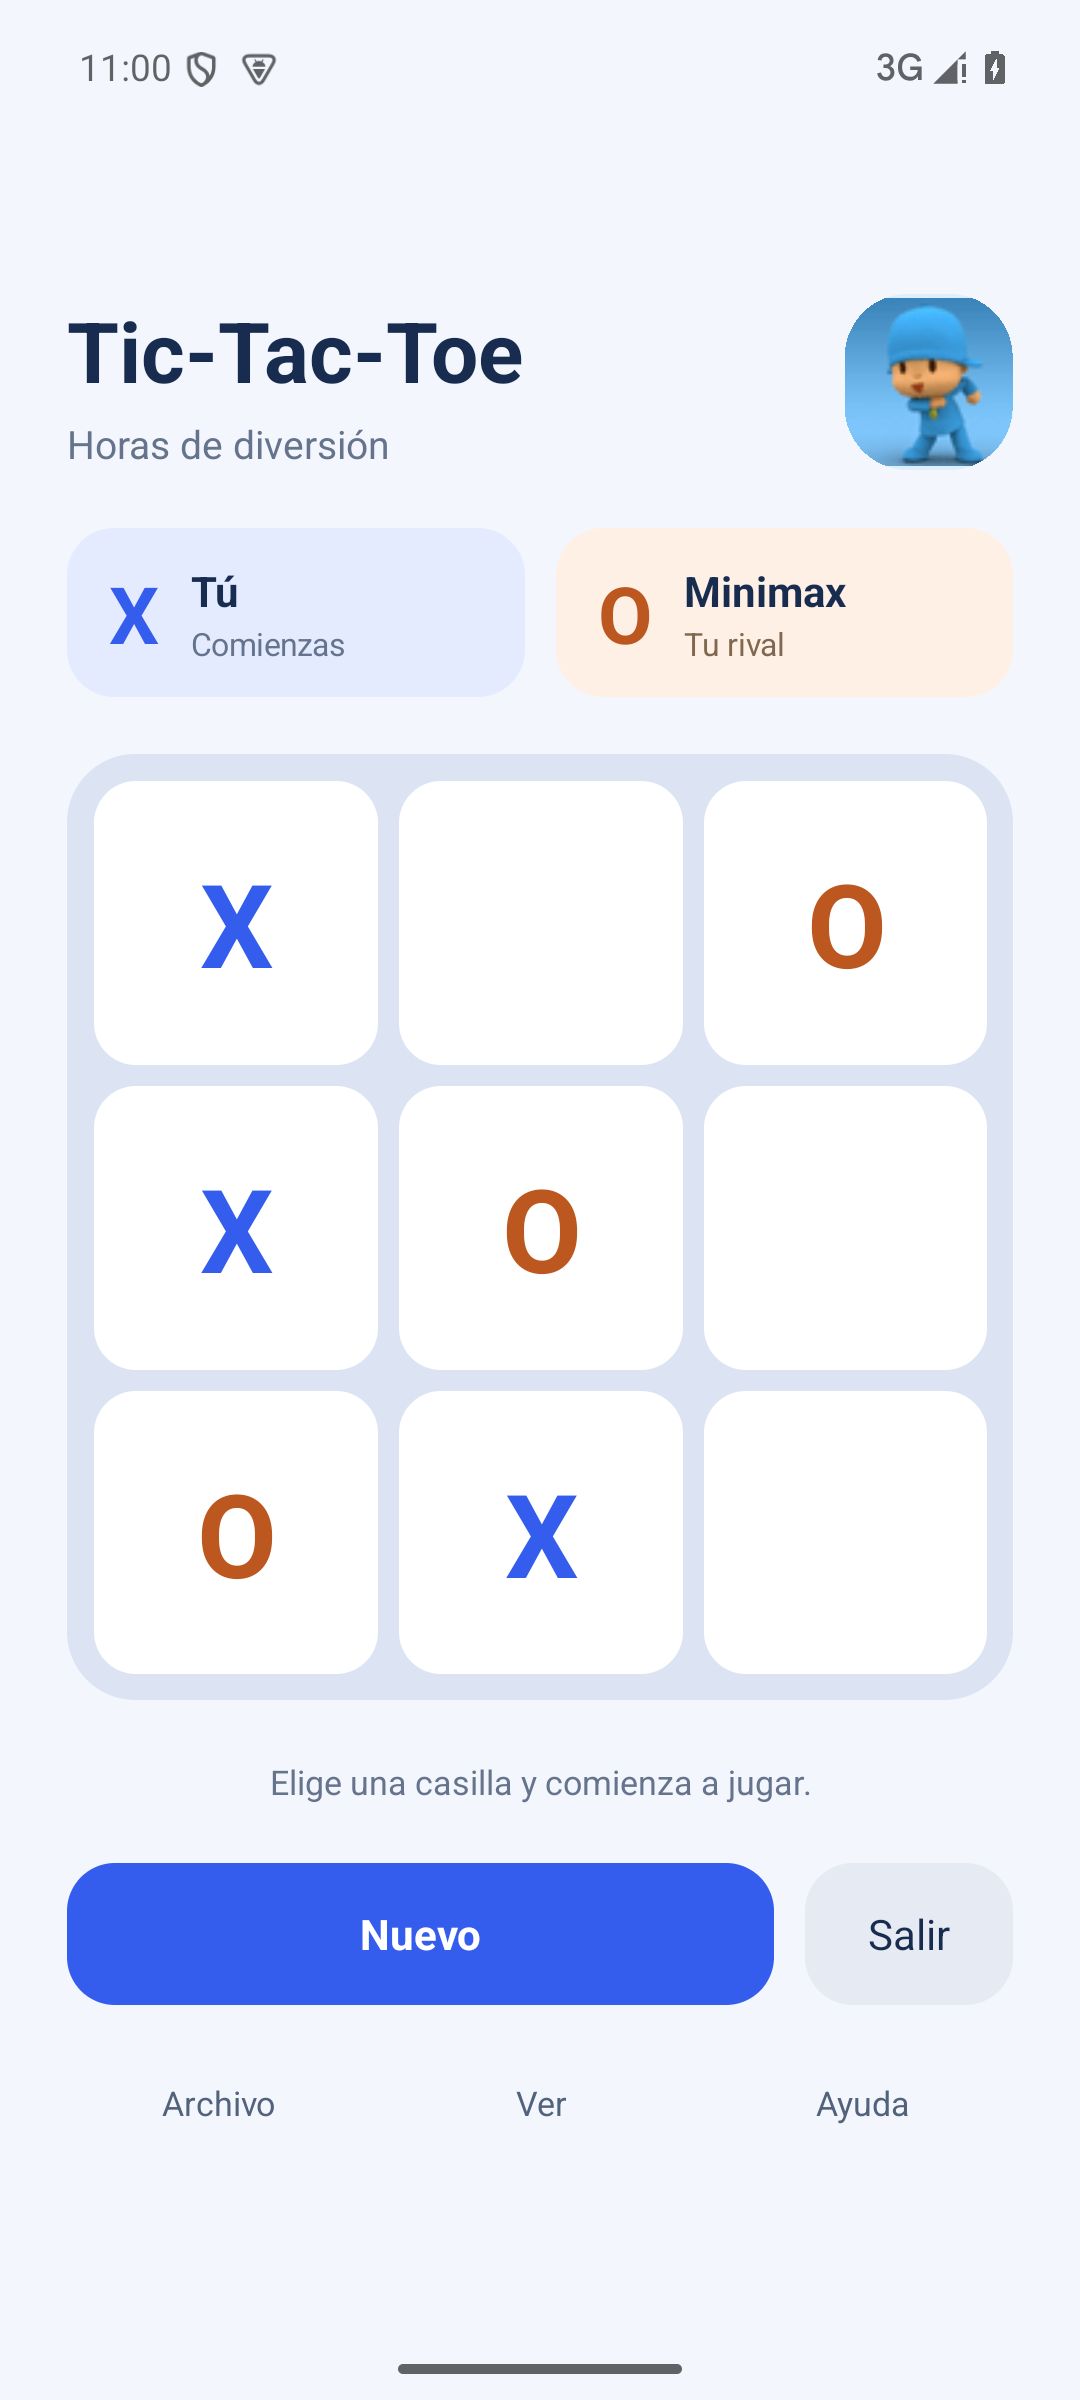
\includegraphics[height=0.78\textheight,keepaspectratio]{figuras/emulador/09_partida_finalizada.png}
\caption{Tablero con victoria diagonal de \texttt{O}; la entrada posterior queda bloqueada.}\label{fig:emu09}
\end{figure}
\clearpage
\begin{figure}[!htbp]\centering
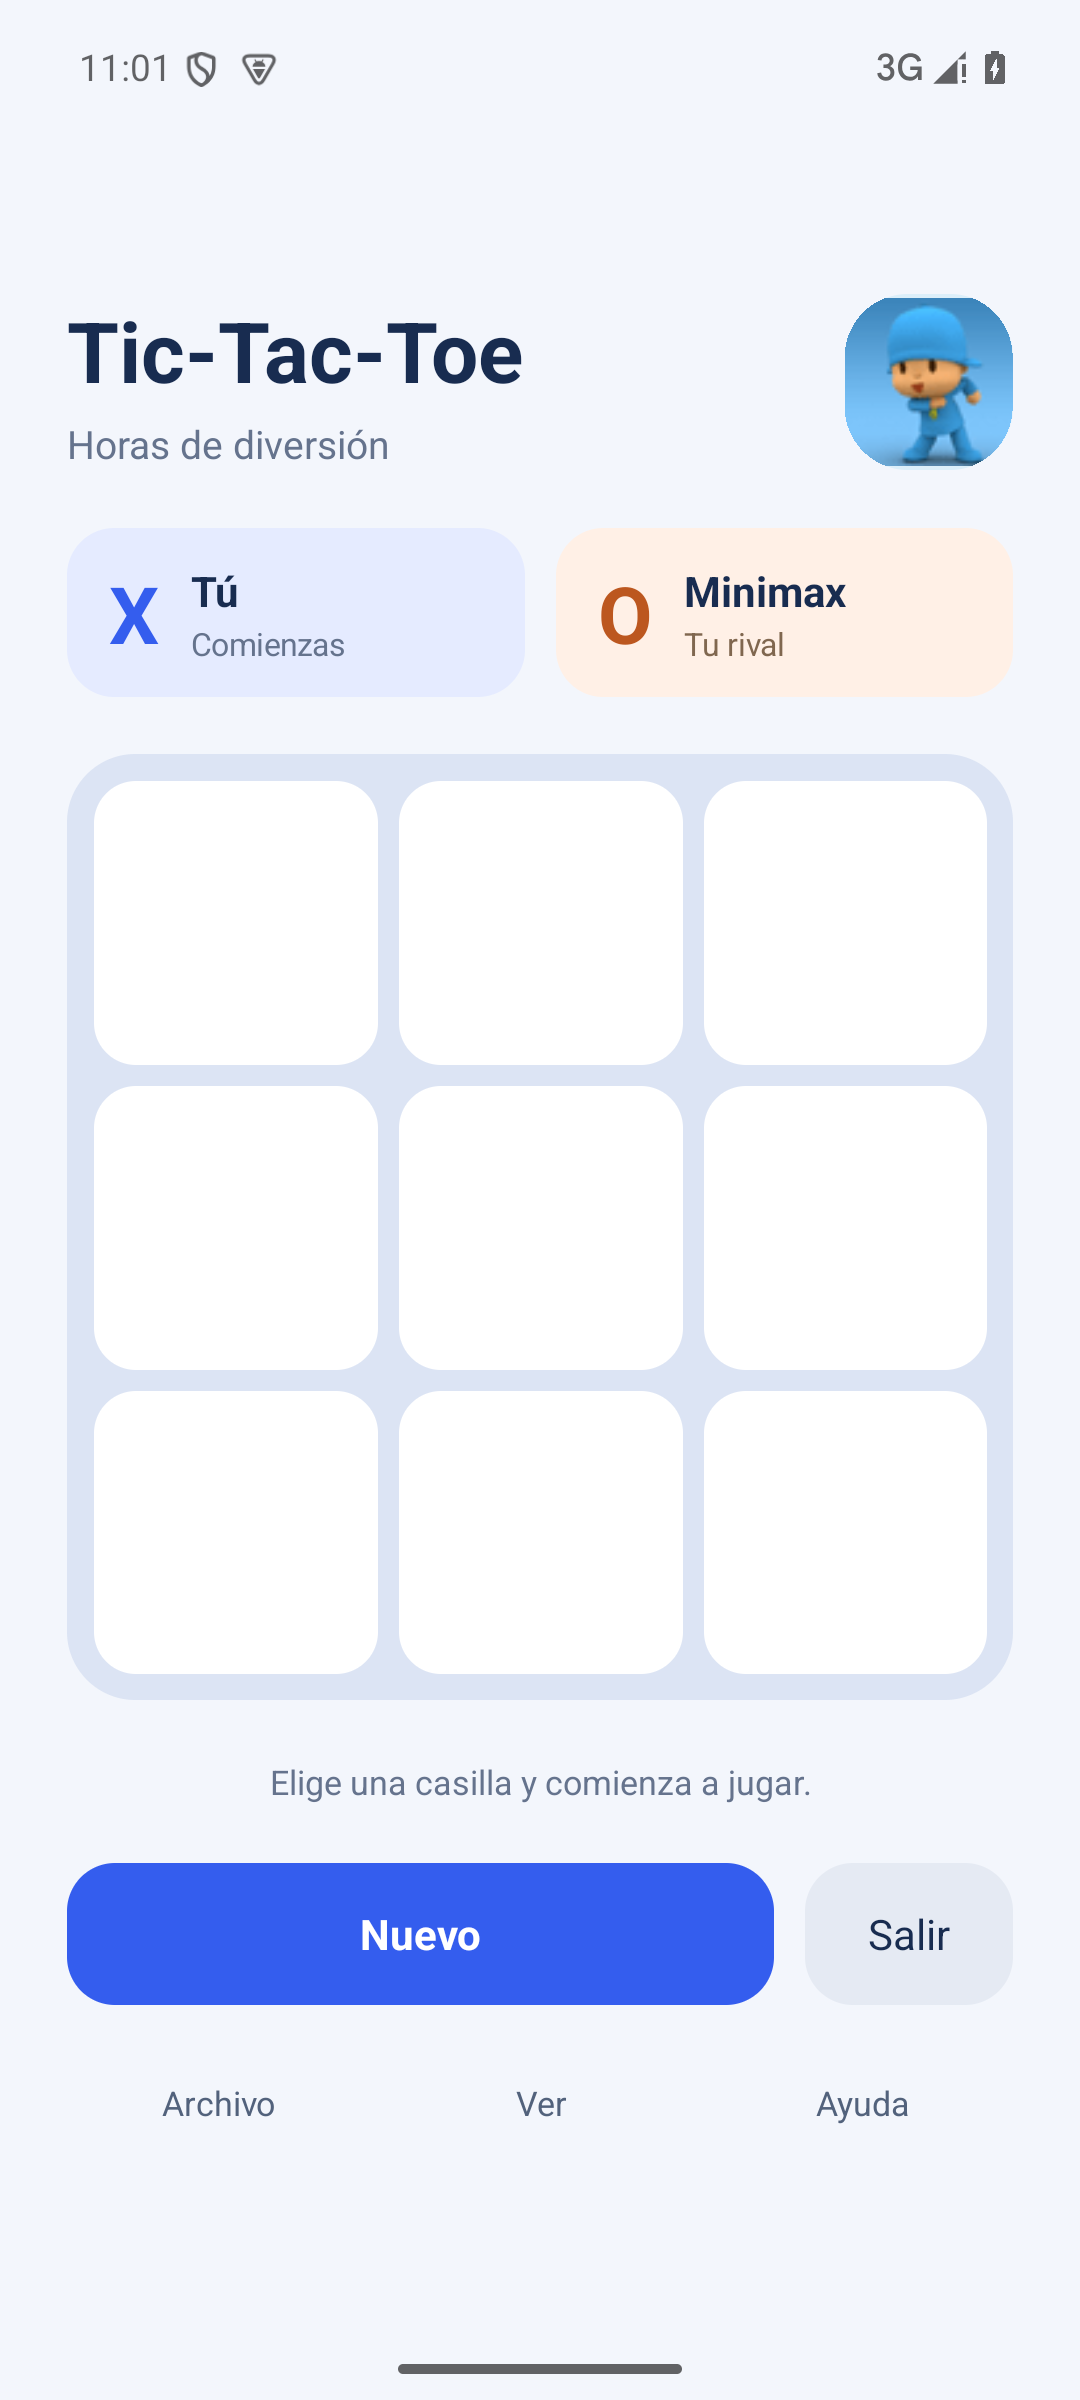
\includegraphics[height=0.78\textheight,keepaspectratio]{figuras/emulador/10_reinicio.png}
\caption{El botón Nuevo limpia la partida y habilita nuevamente las casillas.}\label{fig:emu10}
\end{figure}
\clearpage
\begin{figure}[!htbp]\centering
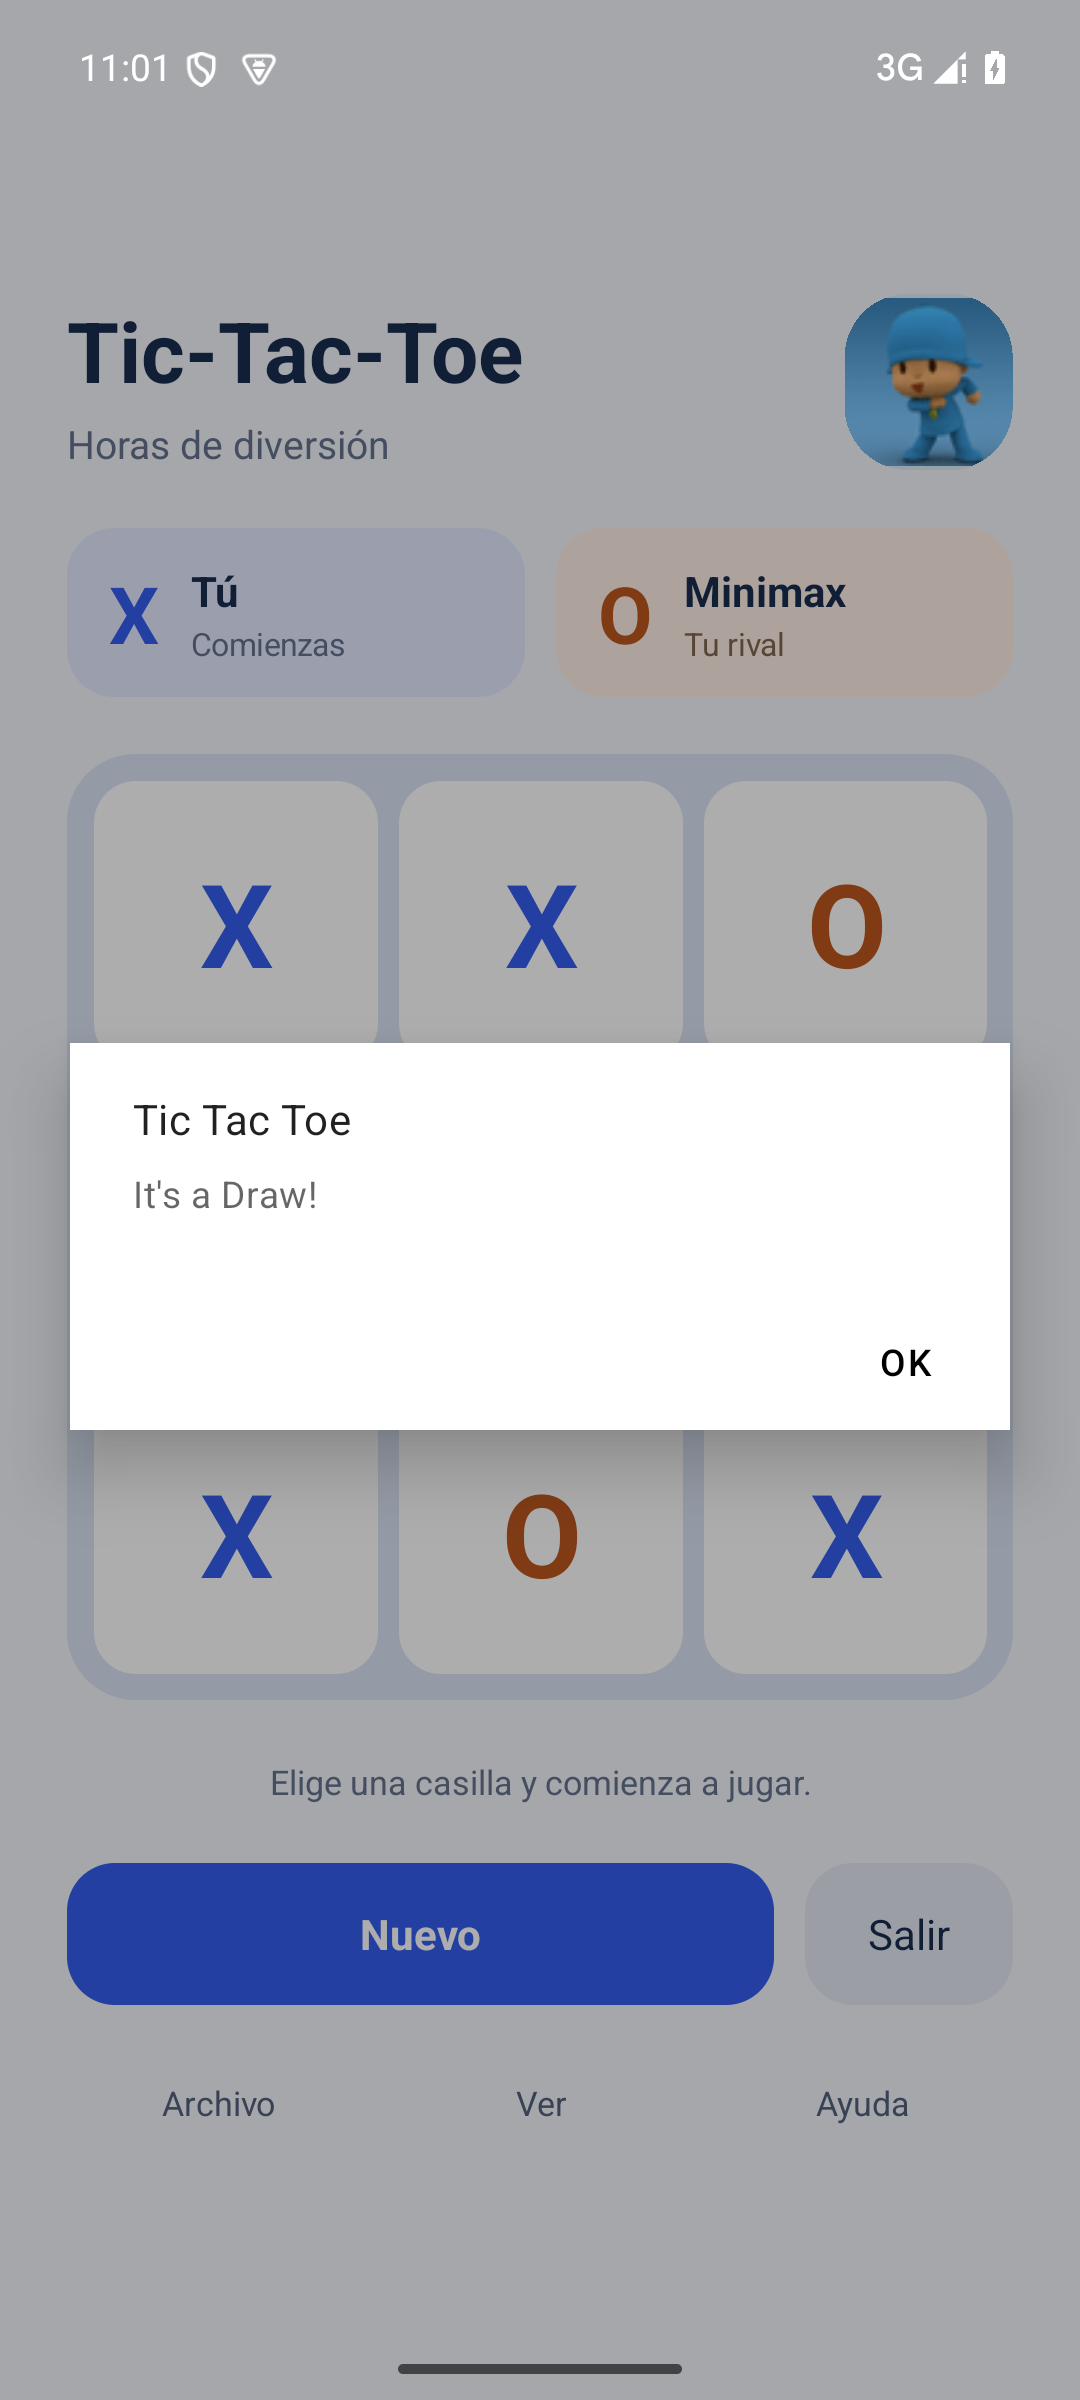
\includegraphics[height=0.78\textheight,keepaspectratio]{figuras/emulador/11_empate_aviso.png}
\caption{Aviso de empate al completar el tablero sin una línea ganadora.}\label{fig:emu11}
\end{figure}
\clearpage
\begin{figure}[!htbp]\centering
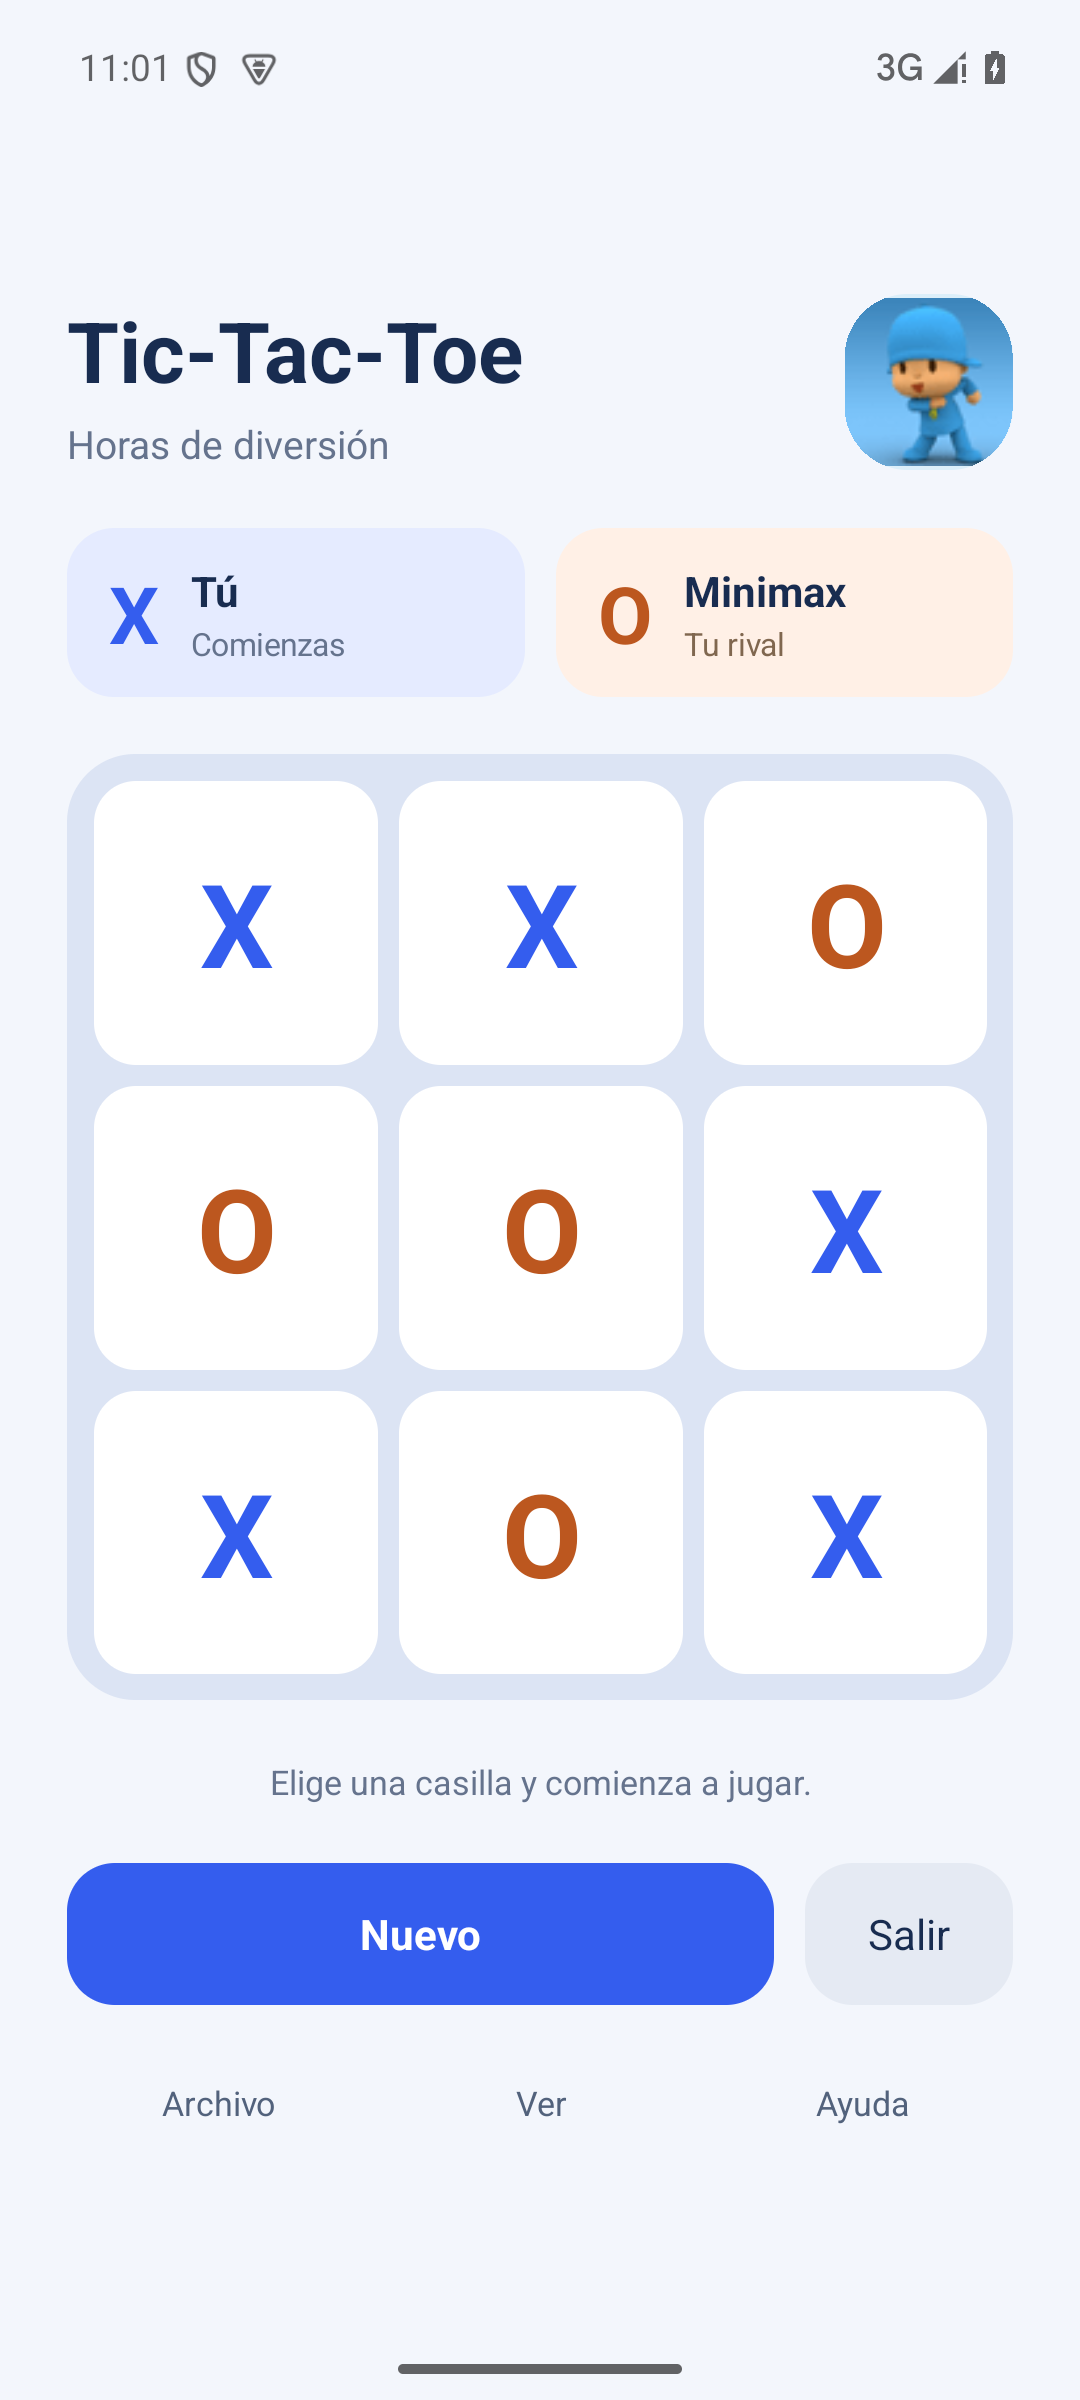
\includegraphics[height=0.78\textheight,keepaspectratio]{figuras/emulador/12_empate_tablero.png}
\caption{Estado final del tablero empatado.}\label{fig:emu12}
\end{figure}
\clearpage
\begin{figure}[!htbp]\centering
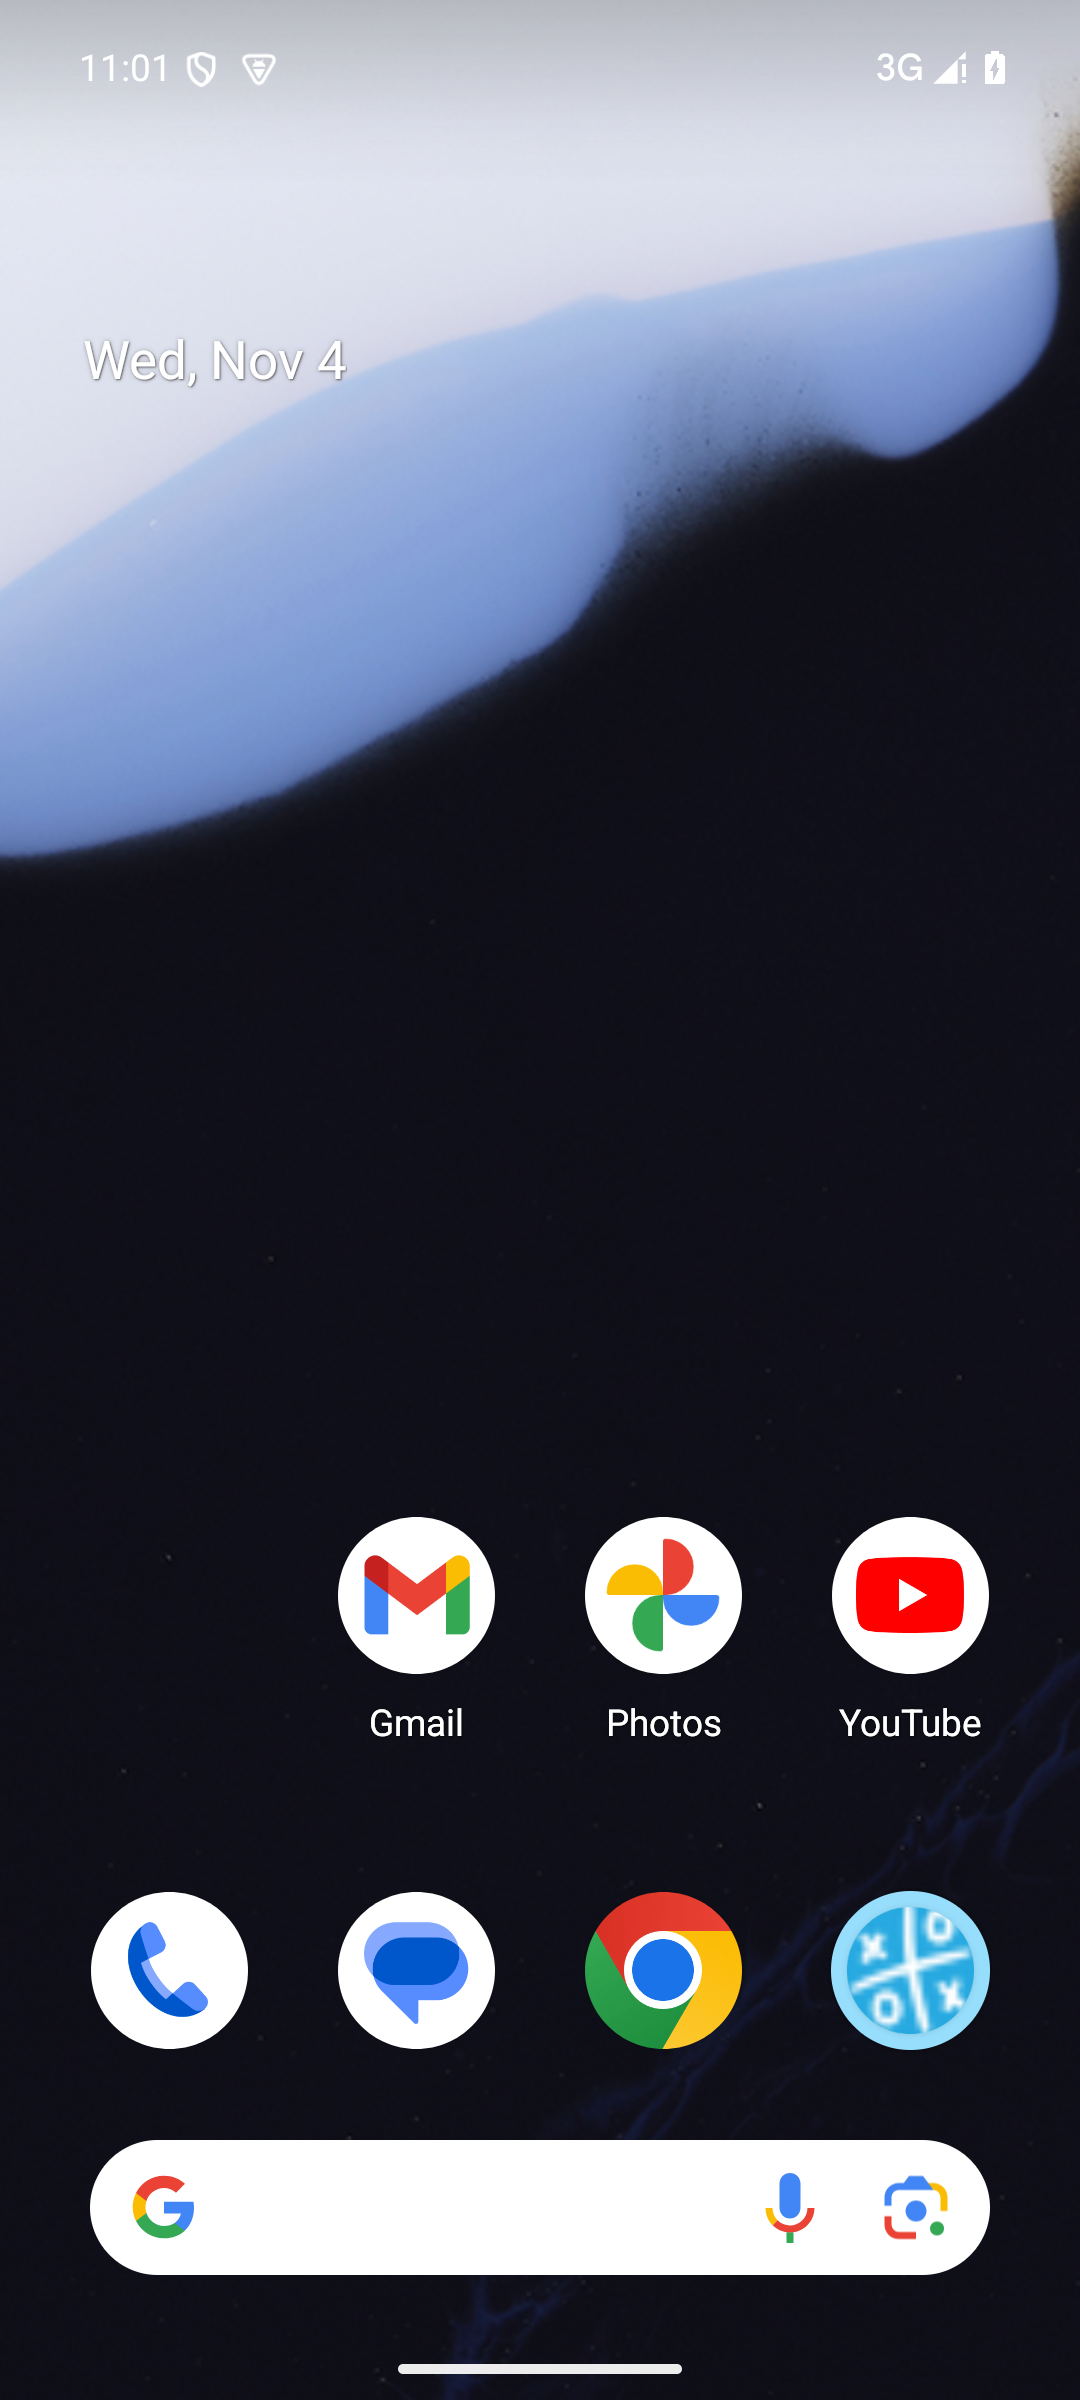
\includegraphics[height=0.78\textheight,keepaspectratio]{figuras/emulador/13_salida.png}
\caption{Pantalla de inicio de Android tras usar el botón Salir.}\label{fig:emu13}
\end{figure}
\clearpage
\begin{figure}[!htbp]\centering
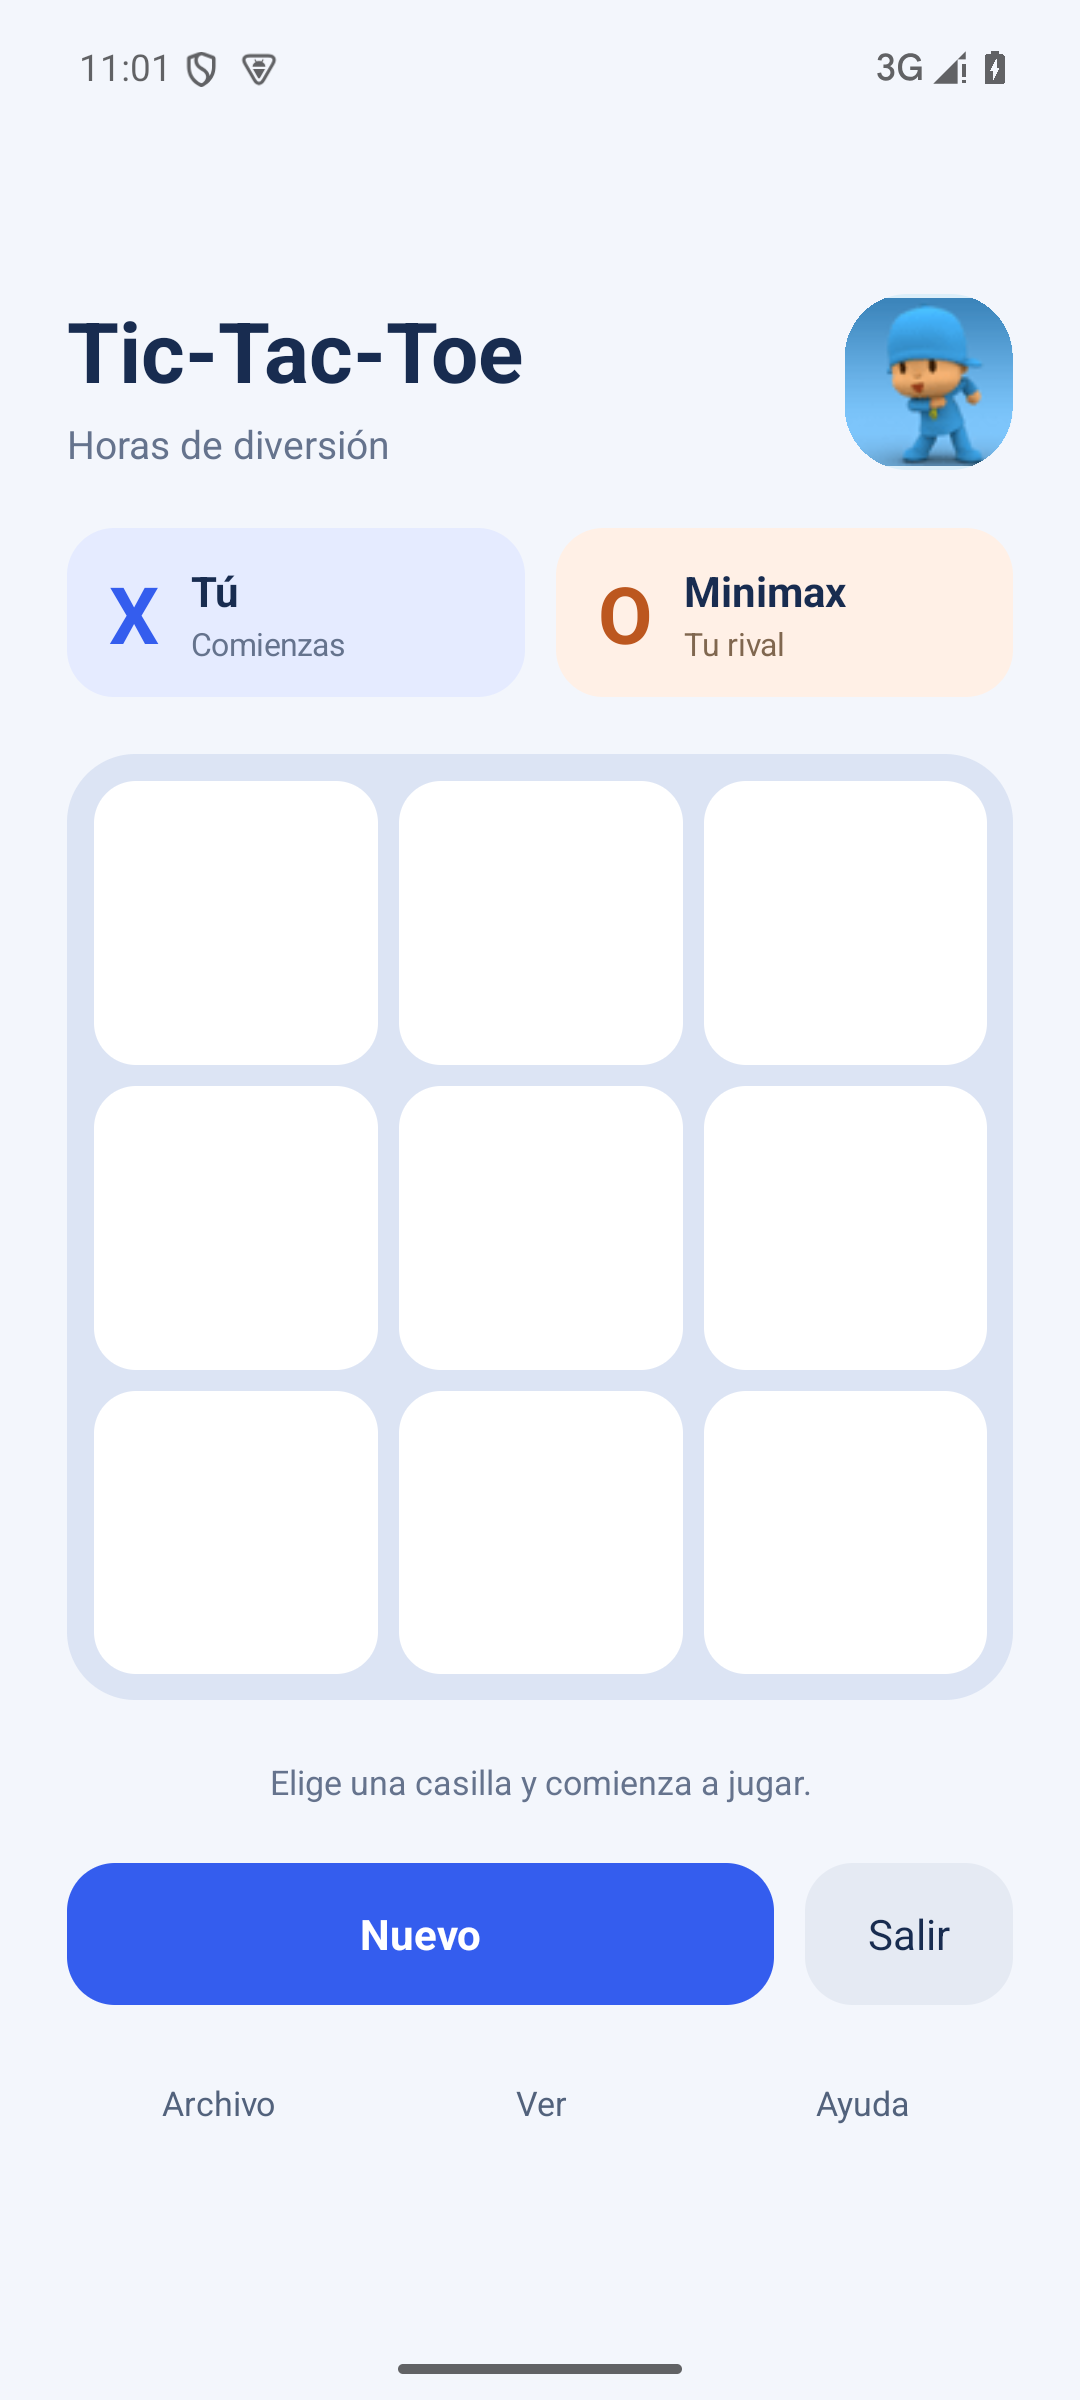
\includegraphics[height=0.78\textheight,keepaspectratio]{figuras/emulador/14_reapertura.png}
\caption{Aplicación reabierta con una partida nueva y tablero vacío.}\label{fig:emu14}
\end{figure}
